%%%%%%%%%%%%%%%%%%%%%%%%%%%%%%%%%%%%%%%%%
% Classicthesis Typographic Thesis
% LaTeX Template
% Version 1.3 (15/2/14)
%
% This template has been downloaded from:
% http://www.LaTeXTemplates.com
%
% Original author:
% André Miede (http://www.miede.de)
%
% License:
% CC BY-NC-SA 3.0 (http://creativecommons.org/licenses/by-nc-sa/3.0/)
%
% General Tips:
% 1) Make sure to edit the classicthesis-config.file
% 2) New enumeration (A., B., C., etc in small caps): \begin{aenumerate} \end{aenumerate}
% 3) For margin notes: \marginpar or \graffito{}
% 4) Do not use bold fonts in this style, it is designed around them
% 5) Use tables as in the examples
% 6) See classicthesis-preamble.sty for useful commands
%
%%%%%%%%%%%%%%%%%%%%%%%%%%%%%%%%%%%%%%%%%

%----------------------------------------------------------------------------------------
%	PACKAGES AND OTHER DOCUMENT CONFIGURATIONS
%----------------------------------------------------------------------------------------

\documentclass[
		twoside,openright,titlepage,numbers=noenddot,headinclude,%1headlines,
                footinclude=true,cleardoublepage=empty,
                BCOR=5mm,paper=a4,fontsize=11pt, % Binding correction, paper type and font size
                ngerman,american, % Languages
                ]{scrreprt} 
                
% Includes the file which contains all the document configurations and packages - make sure to edit this file
%%%%%%%%%%%%%%%%%%%%%%%%%%%%%%%%%%%%%%%%%
% Thesis Configuration File
%
% The main lines to change in this file are in the DOCUMENT VARIABLES
% section, the rest of the file is for advanced configuration.
%
%%%%%%%%%%%%%%%%%%%%%%%%%%%%%%%%%%%%%%%%%

%----------------------------------------------------------------------------------------
%	DOCUMENT VARIABLES
%	Fill in the lines below to enter your information into the thesis template
%	Each of the commands can be cited anywhere in the thesis
%----------------------------------------------------------------------------------------

% Remove drafting to get rid of the '[ Date - classicthesis version 4.0 ]' text at the bottom of every page
\PassOptionsToPackage{eulerchapternumbers,listings, pdfspacing, subfig,beramono,eulermath,parts}{classicthesis}
% Available options: drafting parts nochapters linedheaders eulerchapternumbers beramono eulermath pdfspacing minionprospacing tocaligned dottedtoc manychapters listings floatperchapter subfig
% Adding 'dottedtoc' will make page numbers in the table of contents flushed right with dots leading to them

\newcommand{\myTitle}{Efficiently Exploring Multilevel Data with Recursive Partitioning\xspace}
\newcommand{\mySubtitle}{A Dissertation Proposal\xspace}
\newcommand{\myDegree}{Doktor-Ingenieur (Dr.-Ing.)\xspace}
\newcommand{\myName}{Daniel P. Martin\xspace}
\newcommand{\myProf}{Timo\xspace}
\newcommand{\myOtherProf}{Sara\xspace}
\newcommand{\mySupervisor}{Put name here\xspace}
\newcommand{\myFaculty}{Put data here\xspace}
\newcommand{\myDepartment}{Department of Psychology\xspace}
\newcommand{\myUni}{University of Virginia\xspace}
\newcommand{\myLocation}{Charlottesville, VA\xspace}
\newcommand{\myTime}{January 2015\xspace}
\newcommand{\myVersion}{version 4.0\xspace}

%----------------------------------------------------------------------------------------
%	USEFUL COMMANDS
%----------------------------------------------------------------------------------------

\newcommand{\ie}{i.\,e.}
\newcommand{\Ie}{I.\,e.}
\newcommand{\eg}{e.\,g.}
\newcommand{\Eg}{E.\,g.} 

\newcounter{dummy} % Necessary for correct hyperlinks (to index, bib, etc.)
\providecommand{\mLyX}{L\kern-.1667em\lower.25em\hbox{Y}\kern-.125emX\@}

%----------------------------------------------------------------------------------------
%	PACKAGES
%----------------------------------------------------------------------------------------

\usepackage{lipsum} % Used for inserting dummy 'Lorem ipsum' text into the template

%------------------------------------------------

\usepackage[justification=justified,singlelinecheck=false]{caption} % Left-justify captions for tables and figures

%------------------------------------------------
 
\PassOptionsToPackage{latin9}{inputenc} % latin9 (ISO-8859-9) = latin1+"Euro sign"
\usepackage{inputenc}
 
 %------------------------------------------------

%\PassOptionsToPackage{ngerman,american}{babel}  % Change this to your language(s)
% Spanish languages need extra options in order to work with this template
%\PassOptionsToPackage{spanish,es-lcroman}{babel}
\usepackage{babel}

%------------------------------------------------			

%\PassOptionsToPackage{square,numbers}{natbib}
%\usepackage{natbib}

 %------------------------------------------------

\PassOptionsToPackage{fleqn}{amsmath} % Math environments and more by the AMS 
 \usepackage{amsmath}
 
 %------------------------------------------------

\PassOptionsToPackage{T1}{fontenc} % T2A for cyrillics
\usepackage{fontenc}

%------------------------------------------------

\usepackage{xspace} % To get the spacing after macros right

%------------------------------------------------

\usepackage{mparhack} % To get marginpar right

%------------------------------------------------

\usepackage{fixltx2e} % Fixes some LaTeX stuff 

%------------------------------------------------

\PassOptionsToPackage{smaller}{acronym} % Include printonlyused in the first bracket to only show acronyms used in the text
\usepackage{acronym} % nice macros for handling all acronyms in the thesis

%------------------------------------------------

%\renewcommand*{\acsfont}[1]{\textssc{#1}} % For MinionPro
\renewcommand{\bflabel}[1]{{#1}\hfill} % Fix the list of acronyms

%------------------------------------------------

\PassOptionsToPackage{pdftex}{graphicx}
\usepackage{graphicx} 

%----------------------------------------------------------------------------------------
%	FLOATS: TABLES, FIGURES AND CAPTIONS SETUP
%----------------------------------------------------------------------------------------

\usepackage{tabularx} % Better tables
\setlength{\extrarowheight}{3pt} % Increase table row height
\newcommand{\tableheadline}[1]{\multicolumn{1}{c}{\spacedlowsmallcaps{#1}}}
\newcommand{\myfloatalign}{\centering} % To be used with each float for alignment
\usepackage{caption}
\captionsetup{format=hang,font=small}
\usepackage{subfig}  

%----------------------------------------------------------------------------------------
%	CODE LISTINGS SETUP
%----------------------------------------------------------------------------------------

\usepackage{listings} 
%\lstset{emph={trueIndex,root},emphstyle=\color{BlueViolet}}%\underbar} % for special keywords
\lstset{language=[LaTeX]Tex, % Specify the language for listings here
keywordstyle=\color{RoyalBlue}, % Add \bfseries for bold
basicstyle=\small\ttfamily, % Makes listings a smaller font size and a different font
%identifierstyle=\color{NavyBlue}, % Color of text inside brackets
commentstyle=\color{Green}\ttfamily, % Color of comments
stringstyle=\rmfamily, % Font type to use for strings
numbers=left, % Change left to none to remove line numbers
numberstyle=\scriptsize, % Font size of the line numbers
stepnumber=5, % Increment of line numbers
numbersep=8pt, % Distance of line numbers from code listing
showstringspaces=false, % Sets whether spaces in strings should appear underlined
breaklines=true, % Force the code to stay in the confines of the listing box
%frameround=ftff, % Uncomment for rounded frame
frame=single, % Frame border - none/leftline/topline/bottomline/lines/single/shadowbox/L
belowcaptionskip=.75\baselineskip % Space after the "Listing #: Desciption" text and the listing box
}

%----------------------------------------------------------------------------------------
%	HYPERREFERENCES
%----------------------------------------------------------------------------------------

\PassOptionsToPackage{pdftex,hyperfootnotes=false,pdfpagelabels}{hyperref}
\usepackage{hyperref}  % backref linktocpage pagebackref
\pdfcompresslevel=9
\pdfadjustspacing=1

\hypersetup{
% Uncomment the line below to remove all links (to references, figures, tables, etc)
%draft, 
colorlinks=true, linktocpage=true, pdfstartpage=3, pdfstartview=FitV,
% Uncomment the line below if you want to have black links (e.g. for printing black and white)
%colorlinks=false, linktocpage=false, pdfborder={0 0 0}, pdfstartpage=3, pdfstartview=FitV, 
breaklinks=true, pdfpagemode=UseNone, pageanchor=true, pdfpagemode=UseOutlines,
plainpages=false, bookmarksnumbered, bookmarksopen=true, bookmarksopenlevel=1,
hypertexnames=true, pdfhighlight=/O, urlcolor=webbrown, linkcolor=RoyalBlue, citecolor=webgreen,
%------------------------------------------------
% PDF file meta-information
pdftitle={\myTitle},
pdfauthor={\textcopyright\ \myName, \myUni, \myFaculty},
pdfsubject={},
pdfkeywords={},
pdfcreator={pdfLaTeX},
pdfproducer={LaTeX with hyperref and classicthesis}
%------------------------------------------------
}   

% Need to put apacite down here for it to work
\usepackage{apacite}

%----------------------------------------------------------------------------------------
%	BACKREFERENCES
%----------------------------------------------------------------------------------------

\usepackage{ifthen} % Allows the user of the \ifthenelse command
\newboolean{enable-backrefs} % Variable to enable backrefs in the bibliography
\setboolean{enable-backrefs}{false} % Variable value: true or false

\newcommand{\backrefnotcitedstring}{\relax} % (Not cited.)
\newcommand{\backrefcitedsinglestring}[1]{(Cited on page~#1.)}
\newcommand{\backrefcitedmultistring}[1]{(Cited on pages~#1.)}
\ifthenelse{\boolean{enable-backrefs}} % If backrefs were enabled
{
\PassOptionsToPackage{hyperpageref}{backref}
\usepackage{backref} % to be loaded after hyperref package 
\renewcommand{\backreftwosep}{ and~} % separate 2 pages
\renewcommand{\backreflastsep}{, and~} % separate last of longer list
\renewcommand*{\backref}[1]{}  % disable standard
\renewcommand*{\backrefalt}[4]{% detailed backref
\ifcase #1 
\backrefnotcitedstring
\or
\backrefcitedsinglestring{#2}
\else
\backrefcitedmultistring{#2}
\fi}
}{\relax} 

%----------------------------------------------------------------------------------------
%	AUTOREFERENCES SETUP
%	Redefines how references in text are prefaced for different 
%	languages (e.g. "Section 1.2" or "section 1.2")
%----------------------------------------------------------------------------------------

\makeatletter
\@ifpackageloaded{babel}
{
\addto\extrasamerican{
\renewcommand*{\figureautorefname}{Figure}
\renewcommand*{\tableautorefname}{Table}
\renewcommand*{\partautorefname}{Part}
\renewcommand*{\chapterautorefname}{Chapter}
\renewcommand*{\sectionautorefname}{Section}
\renewcommand*{\subsectionautorefname}{Section}
\renewcommand*{\subsubsectionautorefname}{Section}
}
\addto\extrasngerman{
\renewcommand*{\paragraphautorefname}{Absatz}
\renewcommand*{\subparagraphautorefname}{Unterabsatz}
\renewcommand*{\footnoteautorefname}{Fu\"snote}
\renewcommand*{\FancyVerbLineautorefname}{Zeile}
\renewcommand*{\theoremautorefname}{Theorem}
\renewcommand*{\appendixautorefname}{Anhang}
\renewcommand*{\equationautorefname}{Gleichung}
\renewcommand*{\itemautorefname}{Punkt}
}
\providecommand{\subfigureautorefname}{\figureautorefname} % Fix to getting autorefs for subfigures right
}{\relax}
\makeatother

%----------------------------------------------------------------------------------------

\usepackage{classicthesis} 

%----------------------------------------------------------------------------------------
%	CHANGING TEXT AREA 
%----------------------------------------------------------------------------------------

%\linespread{1.05} % a bit more for Palatino
%\areaset[current]{312pt}{761pt} % 686 (factor 2.2) + 33 head + 42 head \the\footskip
%\setlength{\marginparwidth}{7em}%
%\setlength{\marginparsep}{2em}%

%----------------------------------------------------------------------------------------
%	USING DIFFERENT FONTS
%----------------------------------------------------------------------------------------

%\usepackage[oldstylenums]{kpfonts} % oldstyle notextcomp
%\usepackage[osf]{libertine}
%\usepackage{hfoldsty} % Computer Modern with osf
%\usepackage[light,condensed,math]{iwona}
%\renewcommand{\sfdefault}{iwona}
%\usepackage{lmodern} % <-- no osf support :-(
%\usepackage[urw-garamond]{mathdesign} <-- no osf support :-(

\begin{document}

\frenchspacing % Reduces space after periods to make text more compact

\raggedbottom % Makes all pages the height of the text on that page

\selectlanguage{american} % Select your default language - e.g. american or ngerman

\renewcommand*{\bibname}{References} % Uncomment to change the name of the bibliography
%\setbibpreamble{} % Uncomment to include a preamble to the bibliography - some text before the reference list starts

\pagenumbering{roman} % Roman page numbering prior to the start of the thesis content (i, ii, iii, etc)

\pagestyle{plain} % Suppress headers for the pre-content pages

%----------------------------------------------------------------------------------------
%	PRE-CONTENT THESIS PAGES
%----------------------------------------------------------------------------------------

% Title Page

\begin{titlepage}

\begin{addmargin}[-1cm]{-3cm}
\begin{center}
\large

\hfill
\vfill

\begingroup
\color{Maroon}\spacedallcaps{\myTitle} \\ \bigskip % Thesis title
\endgroup

\spacedlowsmallcaps{\myName} % Your name

\vfill
\mySubtitle \\ \medskip % Thesis subtitle
Department of Psychology \\
University of Virginia \\
Charlottesville, VA \\

\vfill

Proposed Committee: \\
Timo von Oertzen (co-chair) \\
Sara Rimm-Kaufmann (co-chair) \\
Brian Nosek \\
Vivian Wong

\end{center}
\end{addmargin}

\end{titlepage} % Main title page

% Back of the title page

\thispagestyle{empty}

\hfill

\vfill

\noindent\myName: \textit{\myTitle,} \mySubtitle, %\myDegree, 
\textcopyright\ \myTime

% You may wish to do something with the back of the title page, such as including your supervisors, location or time frame of the work. Below is an example of doing so although you may want to tweak it to your liking.

%\bigskip

%\noindent\spacedlowsmallcaps{Supervisors}: \\
%\myProf \\
%\myOtherProf \\ 
%\mySupervisor

%\medskip \\

%\noindent\spacedlowsmallcaps{Location}: \\
%\myLocation

%\medskip \\

%\noindent\spacedlowsmallcaps{Time Frame}: \\
%\myTime
 % Back of the title page

%\cleardoublepage\include{FrontBackMatter/Dedication} % Dedication page

%\cleardoublepage\include{FrontBackMatter/Foreword} % Uncomment and create a Foreword.tex to include a foreword

% Abstract

\pdfbookmark[1]{Abstract}{Abstract} % Bookmark name visible in a PDF viewer

\begingroup
\let\clearpage\relax
\let\cleardoublepage\relax
\let\cleardoublepage\relax

\chapter*{Abstract} % Abstract name

	There is an increasing number of data sets with many participants, many variables, or both, found in education and other areas that commonly have complex, multilevel data structures. Once initial confirmatory hypotheses are exhausted, it can be difficult to determine how best to explore these data sets to discover hidden relationships that could help to inform future research. Typically, exploratory data analysis in these areas are performed with the very same statistical tools as confirmatory data analysis, leading to potential methodological issues such as increased rates of false positive findings. In this dissertation proposal, I argue that the utilization of a data mining framework known as recursive partitioning offers a more efficient means to perform exploratory data analysis to identify variables that may have been overlooked initially in the confirmatory data analaysis phase. By adopting such a non-parametric approach, researchers can easily identify the extent to which all variables are related to an outcome, rather than rely on null hypothesis significance tests as a strict dichotomization of whether a given variable is ``important'' or ``unimportant.'' This proposal seeks to evaluate the feasibility of using these methods in multilevel contexts commonly found in social science research by using both Monte Carlo simulations and three applied data sets. Based on these results, a set of best practices will be constructed and disseminated via a small workshop given to applied researchers. Feedback from these researchers will help lead to a publicly available tutorial and R package to assist others interested in adding this technique to their own statistical toolbox.

\endgroup			

\vfill % Abstract page

%\cleardoublepage\include{FrontBackMatter/Publication} % Publications from the thesis page

%\cleardoublepage\include{FrontBackMatter/Acknowledgments} % Acknowledgements page

\pagestyle{scrheadings} % Show chapter titles as headings

% Table of Contents - List of Tables/Figures/Listings and Acronyms

\refstepcounter{dummy}

\pdfbookmark[1]{\contentsname}{tableofcontents} % Bookmark name visible in a PDF viewer

\setcounter{tocdepth}{2} % Depth of sections to include in the table of contents - currently up to subsections

\setcounter{secnumdepth}{3} % Depth of sections to number in the text itself - currently up to subsubsections

\manualmark
\markboth{\spacedlowsmallcaps{\contentsname}}{\spacedlowsmallcaps{\contentsname}}
\tableofcontents 
\automark[section]{chapter}
\renewcommand{\chaptermark}[1]{\markboth{\spacedlowsmallcaps{#1}}{\spacedlowsmallcaps{#1}}}
\renewcommand{\sectionmark}[1]{\markright{\thesection\enspace\spacedlowsmallcaps{#1}}}

\clearpage

\begingroup 
\let\clearpage\relax
\let\cleardoublepage\relax
\let\cleardoublepage\relax

%----------------------------------------------------------------------------------------
%	List of Figures
%----------------------------------------------------------------------------------------

\refstepcounter{dummy}
%\addcontentsline{toc}{chapter}{\listfigurename} % Uncomment if you would like the list of figures to appear in the table of contents
\pdfbookmark[1]{\listfigurename}{lof} % Bookmark name visible in a PDF viewer

\listoffigures

\vspace*{8ex}
\newpage

%----------------------------------------------------------------------------------------
%	List of Tables
%----------------------------------------------------------------------------------------

\refstepcounter{dummy}
%\addcontentsline{toc}{chapter}{\listtablename} % Uncomment if you would like the list of tables to appear in the table of contents
\pdfbookmark[1]{\listtablename}{lot} % Bookmark name visible in a PDF viewer

\listoftables
        
\vspace*{8ex}
\newpage
       
%----------------------------------------------------------------------------------------
%	Acronyms
%----------------------------------------------------------------------------------------

%\refstepcounter{dummy}
%\addcontentsline{toc}{chapter}{Acronyms} % Uncomment if you would like the acronyms to appear in the table of contents
%\pdfbookmark[1]{Acronyms}{acronyms} % Bookmark name visible in a PDF viewer

%\markboth{\spacedlowsmallcaps{Acronyms}}{\spacedlowsmallcaps{Acronyms}}

%\chapter*{Acronyms}

                   
\endgroup % Contents, list of figures/tables/listings and acronyms

\cleardoublepage

\pagenumbering{arabic} % Arabic page numbering for thesis content (1, 2, 3, etc)
%\setcounter{page}{90} % Uncomment to manually start the page counter at an arbitrary value (for example if you wish to count the pre-content pages in the page count)

\cleardoublepage % Avoids problems with pdfbookmark

%----------------------------------------------------------------------------------------
%	THESIS CONTENT - CHAPTERS
%----------------------------------------------------------------------------------------

% Chapter 1

\chapter{Introduction} % Chapter title

\label{ch:introduction} % For referencing the chapter elsewhere, use \autoref{ch:introduction} 

% Intro text

\begin{flushleft}{\slshape    
Once upon a time statisticians only explored. Then they learned to \\
confirm exactly - to confirm a few things exactly, each under very \\
specific circumstances. As they emphasized exact confirmation, their \\
techniques inevitably became less flexible. The connection of the most \\
used techniques with past insights was weakened. Anything to which \\
a confirmatory procedure was not explicitly attached was decried as \\
'mere descriptive statistics', no matter how much we had learned from it.} \\ \medskip
--- \citeA{tukey1977exploratory}
\end{flushleft}

\bigskip

Consider the following scenario: An educational researcher just finished collecting data for a large grant examining how teacher-student interactions are related to student outcomes. When originally writing up the grant, the researcher had some specific hypotheses grounded in theory that the grant was designed to test. The data set was cleaned and prepped, and the hypotheses were empirically tested. These tests yielded results providing support for some of the original hypotheses, while others were a little less clear. Naturally, the researcher had collected additional variables that may or may not be relevant to the outcome (e.g., teacher and student demographics), and is now interested in performing exploratory data analysis to examine these variables further. However, unlike the original hypotheses, theory does not have strong predictions for these additional variables. Interested in performing a more exploratory study with these data, the researcher now has to make decisions regarding which variables to include, how these variables might be related (linearly, quadratically, etc.), and if potential interactions might be necessary in these exploratory models. How does the researcher proceed?


This situation is becoming more common as there is an increasing number of datasets with a large number of participants, variables, or both, in education and other fields that often deal with multilevel data structures. With this increase of available information, it becomes necessary to be able to efficiently search a large parameter space to identify variables that might have been overlooked to uncover insights and help inform future research. Currently, this practice is typically accomplished in the social sciences ``by hand.'' That is, the researcher in question will run multiple tests from a hypothesis testing framework with different model specifications and combinations of variables in order to determine which are the most important \cite{strobl2009introduction}.


While some argue that exploratory approaches do not need any type of correction as the results are preliminary \cite{schochet2008technical}, performing exploratory data analysis solely with a hypothesis testing framework is still rife with statistical issues regarding the generalizability of such findings. For example, it is easy to blur the lines between what is confirmatory and what is exploratory when confronted with a large dataset with many possible quantitative decisions \cite{wagenmakers2012agenda}. In such situations, there is an increased chance of detecting spurious findings due to the large number of potential researcher degrees of freedom \cite{gelman2014statistical, ioannidis2005most, simmons2011false}. Even seemingly simple choices of what covariates to include or which distribution to specify for the outcome is enough to make researchers come to different conclusions regarding the statistical significance of a given variable when confronted with the same research question \cite{silberzahn2014}.


To address this concern, more emphasis is being placed on replication \cite{osc2014, oscinpress}. Although many participating in this movement stem from social psychology in particular, this movement has also been echoed in other areas where complex multilevel data are commonplace, such as developmental psychology \cite{duncan2014} and education \cite{makel2014facts}. While replicability is a hallmark of good scientific practice \cite{nosek2012scientific}, it is more feasible to implement as a means to control for potential spurious effects caused by a large number of researcher degrees of freedom in some domains more than others \cite{finkelinpress}. In many social psychology lab studies, for example, the preliminary nature of exploratory data analysis can simply be confirmed with the running of additional studies at relatively minimal cost. Studies that are run in settings as complex as a school system unfortunately do not have this luxury. 


What is needed, then, is a more efficient means of exploratory data analysis that can help uncover insight while simultaneously controlling for spurious findings, have the ability to be implemented when theory might not dictate how the model should be specified, handle situations where complex, multilevel data structures are commonplace, and, arguably most important, be something that can be adopted by the average, applied researcher. Given that previous research has focused solely on performing confirmatory and exploratory research from a null hypothesis significance testing perspective \cite{berk2008statistical, finkelinpress}, identifying a potential solution to this problem seems almost infeasible. However, solutions are readily available with a simple, two-step shift in statistical perspective. 

First, focus needs to be placed on predictive modeling (i.e., predicting new observations based on patterns found in previous observations) rather than explanatory modeling (i.e., providing evidence for a hypothesis with significant effects in a given direction). This removes the burden of using existing theory (which may or may not exist) to dictate what should or should not be specified in a given statistical model \cite{shmueli2010explain}. The second step involves utilizing algorithmic methods that assume the data generative mechanism is unknown, rather than adopting a method that relies on the assumption that the data were generated from a given stochastic model \cite{breiman2001statistical}. In other words, instead of assuming that the relation between an outcome and a predictor is a specific function of the given predictor value, its estimated parameter, and random noise, an algorithm treats the functional relation between the predictor and the outcome as unknown and something to be estimated. Algorithmic methods remove the burden of specifying complex function forms, such as non-linear relations or higher order interactions, when attempting to build predictive data models.


Through this shift of perspective, it becomes possible to understand and adopt a popular data mining algorithm known as recursive partitioning to identify subsets of variables that are most related to a given outcome, and what kind of statistical relation it might be. This framework produces a set of binary decision rules based on covariate values in an attempt to create a set of subgroups, or nodes, which are homogeneous with respect to a given outcome \cite{mcardle2013}. This is particularly relevant in the context of multilevel data, where cases or observations are nested (e.g., children nested within classrooms). In these situations, using traditional methods, such as linear regression, can result in an increased chance of detecting significant effects due to the broken statistical assumption of independence \cite{peugh2010practical}. The general recursive partitioning framework, on the other hand, makes no such assumptions, indicating that this method could extend to multilevel data structures with little added complications. And yet despite its potential utility in the social sciences, the implementation of these algorithms in the face of complex, multilevel data structures, is not well understood \cite{mcardle2013}.


The purpose of this dissertation is to evaluate the implementation of two popular recursive partitioning algorithms in the presence of multilevel data structures commonly found in applied educational and psychological contexts. Upon finishing this dissertation, I will be able to conclude whether recursive partitioning is a feasible tool to conduct exploratory data analysis in the presence of multilevel data, and, if so, which underlying algorithm yields the best results. This proposal is structured into five chapters. \autoref{ch:methods} provides a foundational overview of the two popular algorithms under investigation, classification and regression trees (CART) and conditional inference trees (CTREE), as well as their ensemble method (i.e., forest) counterparts. This section also includes a brief overview of statistical terminology relevant to understanding the application of predictive models, such as bias, variance, and model validation. \autoref{ch:previous} covers previous research extending recursive partitioning frameworks to more advanced applications relevant to complex, multilevel data structures. \autoref{ch:problem} outlines unanswered questions when considering the application of both CART or CTREE to multilevel data structures, with a set of hypotheses based on previous research and preliminary simulation results. \autoref{ch:proposal} is the proposal. This section includes how the open questions proposed in \autoref{ch:problem} will be evaluated with a proposed simulation study. Additionally, this section will outline three large, multilevel datasets to be explored with recursive partitioning as well as plans to disseminate a set of best practices for applied researchers interested in these methods for their own research.

 % Chapter 1
% Chapter 2

\chapter{Recursive partitioning and ensemble methods} % Chapter title

\label{ch:methods} % For referencing the chapter elsewhere, use \autoref{ch:methods} 


	Recursive partitioning is a non-parametric, data-driven statistical algorithm that iteratively searches a given predictor space to identify potential splits, thus segmenting the space into distinct, rectangular subsections. Then, a simple model, most often a constant, is fit in each one \cite{hastie2009elements}. In the case of a continuous outcome, this recursive partitioning procedure is referred to as a \textit{regression tree}, and the constant reflects the mean value of all observations in a given subsection. Otherwise, if the outcome is categorical, it is referred to as a \textit{classification tree}, and the constant is assigned to be the specific category with the highest frequency over all observations in the particular subsection. As such, recursive partitioning is not limited to a binary outcome, but can actually model an outcome with $K$ potential classes.


	This framework was initially formulated through the seminal work of \citeA{morgan1963problems}, who proposed focusing on predictive accuracy in large survey data as a means to relax additive assumptions commonly made at that time in order to detect complex relations among predictor variables; a process they referred to as Automatic Interaction Detection. This framework was further solidified by both \citeA{breiman1984classification} and \citeA{quinlan1986induction}, who created algorithms seeking to improve on this original idea. Initially, recursive partitioning was met with much disdain by the statistics community due to its poor generalizability, especially when inappropriately applied to small data sets with large noise-to-signal ratios \cite{hastie2013}. However, this recently changed in the past decade or two, when the work of \citeA{breiman1984classification} started to become widely adopted as a useful tool in predictive modeling. Still, this method is relatively unknown to those in the social sciences \cite{mcardle2013}.


	Given the immense popularity of the recursive partitioning framework, it is no surprise that many algorithms exist, each with their own advantages and disadvantages. This dissertation focuses on two of the most widely used recursive partitioning algorithms: classification and regression trees \cite<CART;>{breiman1984classification} and conditional inference trees \cite<CTREE;>{hothorn2006unbiased}. These two algorithms, in addition to other important concepts inherent in predictive modeling, are described below. To assist in this overview and to highlight how the methods are used in practice, a data set examining the relation between graduation rates and various statistics for US Colleges (N = 777) from the 1995 issue of US News and World Report will be used. This data set is freely available from the ISLR package \cite{ISLRR} in the R software environment \cite{Rcore}, and contains 17 variables that can be used as predictors for graduation rate, such as whether a university is private or public, the acceptance rate, and the out-of-state tuition cost. 


%----------------------------------------------------------------------------------------

\section{Classification and regression trees}


	Originally proposed by \citeA{breiman1984classification}, CART is easily the most popular and widely used recursive partitioning algorithm, being cited almost 26,000 times according to Google Scholar\footnote{As of November 13, 2014}. When initially creating a decision tree, the algorithm consists of essentially four steps \cite{james2013introduction}. First, all predictor variables are initially considered for potential splits in a \textit{greedy}, \textit{top-down} manner. The splitting process is greedy, because each step searches for the best possible split at that time, rather than considering previous or future steps. It is top-down, because it begins with all observations belonging to the same group, or node, and then subsequently conducts splits further down the tree after initial splits have been made. Second, the best potential split is identified by some criterion, which is taken to be the residual sums of squares (RSS) in the case of a continuous outcome. Following the notation of \citeA{hastie2009elements}, suppose we have a predictor variable $X_j$ with a given split point $s$, which splits the predictor space into two regions: $R_1(j, s) = \left\{ X \mathrel{}\middle|\mathrel{} X_j < s\right\}$ and $R_2(j, s) = \left\{ X \mathrel{}\middle|\mathrel{} X_j \geq s\right\}$. The algorithm searches for a particular $j$ and $s$ that minimizes the following equation:

\begin{equation} 
\sum_{i: x_i \in R_1(j, s)} (y_i - \hat{y}_{R_1})^2 + \sum_{i: x_i \in R_2(j, s)} (y_i - \hat{y}_{R_2})^2
\end{equation}

\noindent where $\hat{y}_{R_j}$ is the mean of the outcome within the $j$th subsection and $\sum_{i: x_i \in R_j(j, s)} (y_i - \hat{y}_{R_j})^2$ is the RSS over all $i$ participants in the $j$th subsection.

	Once the best split is identified, the data is split on this threshold, creating two new subsections, or \textit{child nodes}. The same procedure outlined above is then performed separately on each of these nodes, and this process is repeated until some stopping criterion is reached. For example, the algorithm might require a minimum number of observations to belong to a given node, regardless of whether another split will result in a reduction of the RSS. Finally, the given node becomes a \textit{terminal node} once no further splits can be made within that node. When all nodes can no longer be split any further due to these stopping criteria, the algorithm terminates. 

	See \autoref{fig:exampletree} for an example decision tree might look in the college graduation rate data set. The corresponding decision tree first splits on the out-of-state tuition variable, which is a variable reflecting the annual tuition cost a student has to pay to attend the institution when they live in a different state (range: \$2340 - \$21700). This decision creates a vertical line in two-dimensional space, splitting the data into two subsections at approximately \$10,000. Both of these nodes are again split by the out-of-state tuition variable, resulting in two more lines being drawn and creating four subsections in total. Finally, one node is further split by the percentage of students at an institution who were in the top ten percent of their high school class, resulting in a horizontal line creating a fifth subsection. Note that only two variables were used in the splitting process to maintain interpretability with the corresponding visualization.


\begin{figure}
\begin{tabular}{c}
\subfloat[]{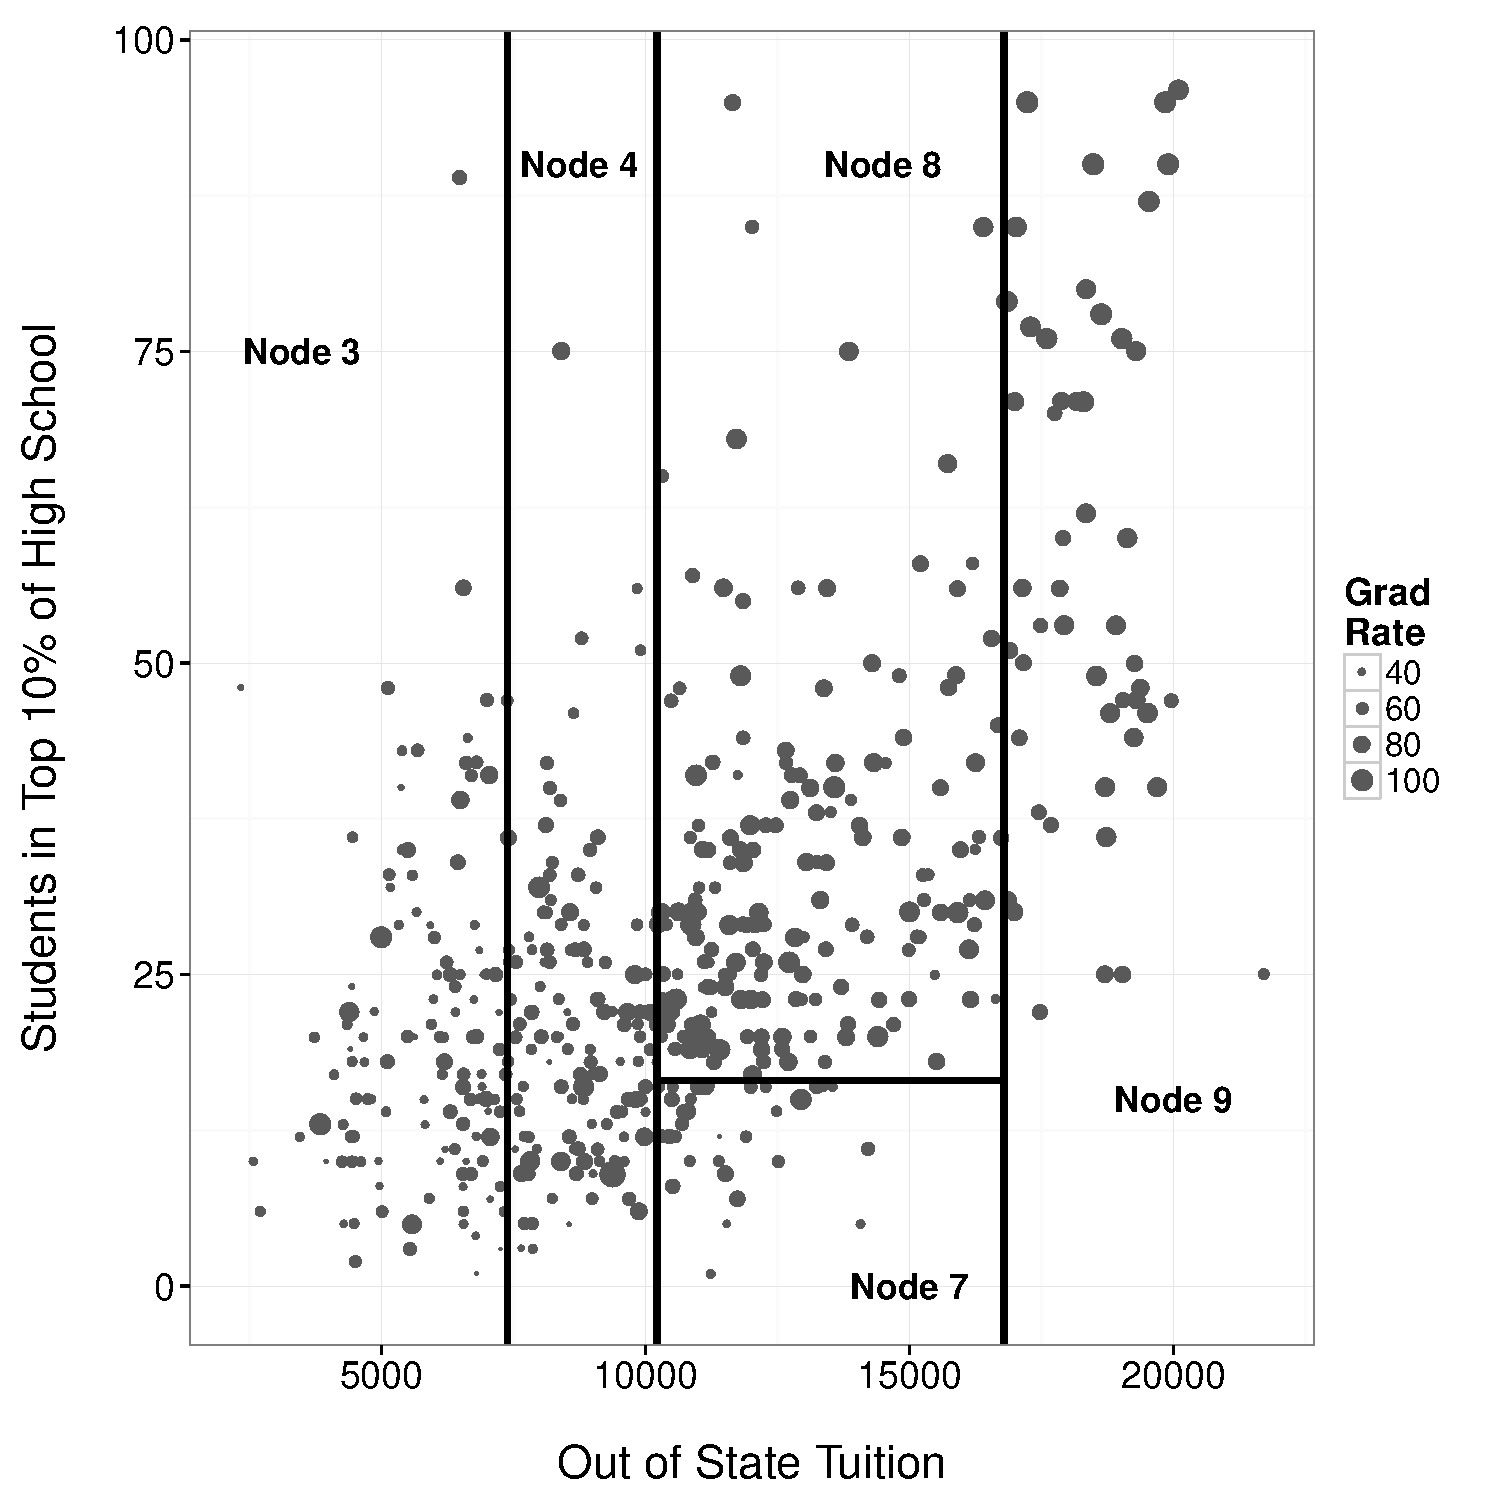
\includegraphics[width = 3.5in]{Figures/Chapter02/part_plot.pdf}} \\
\subfloat[]{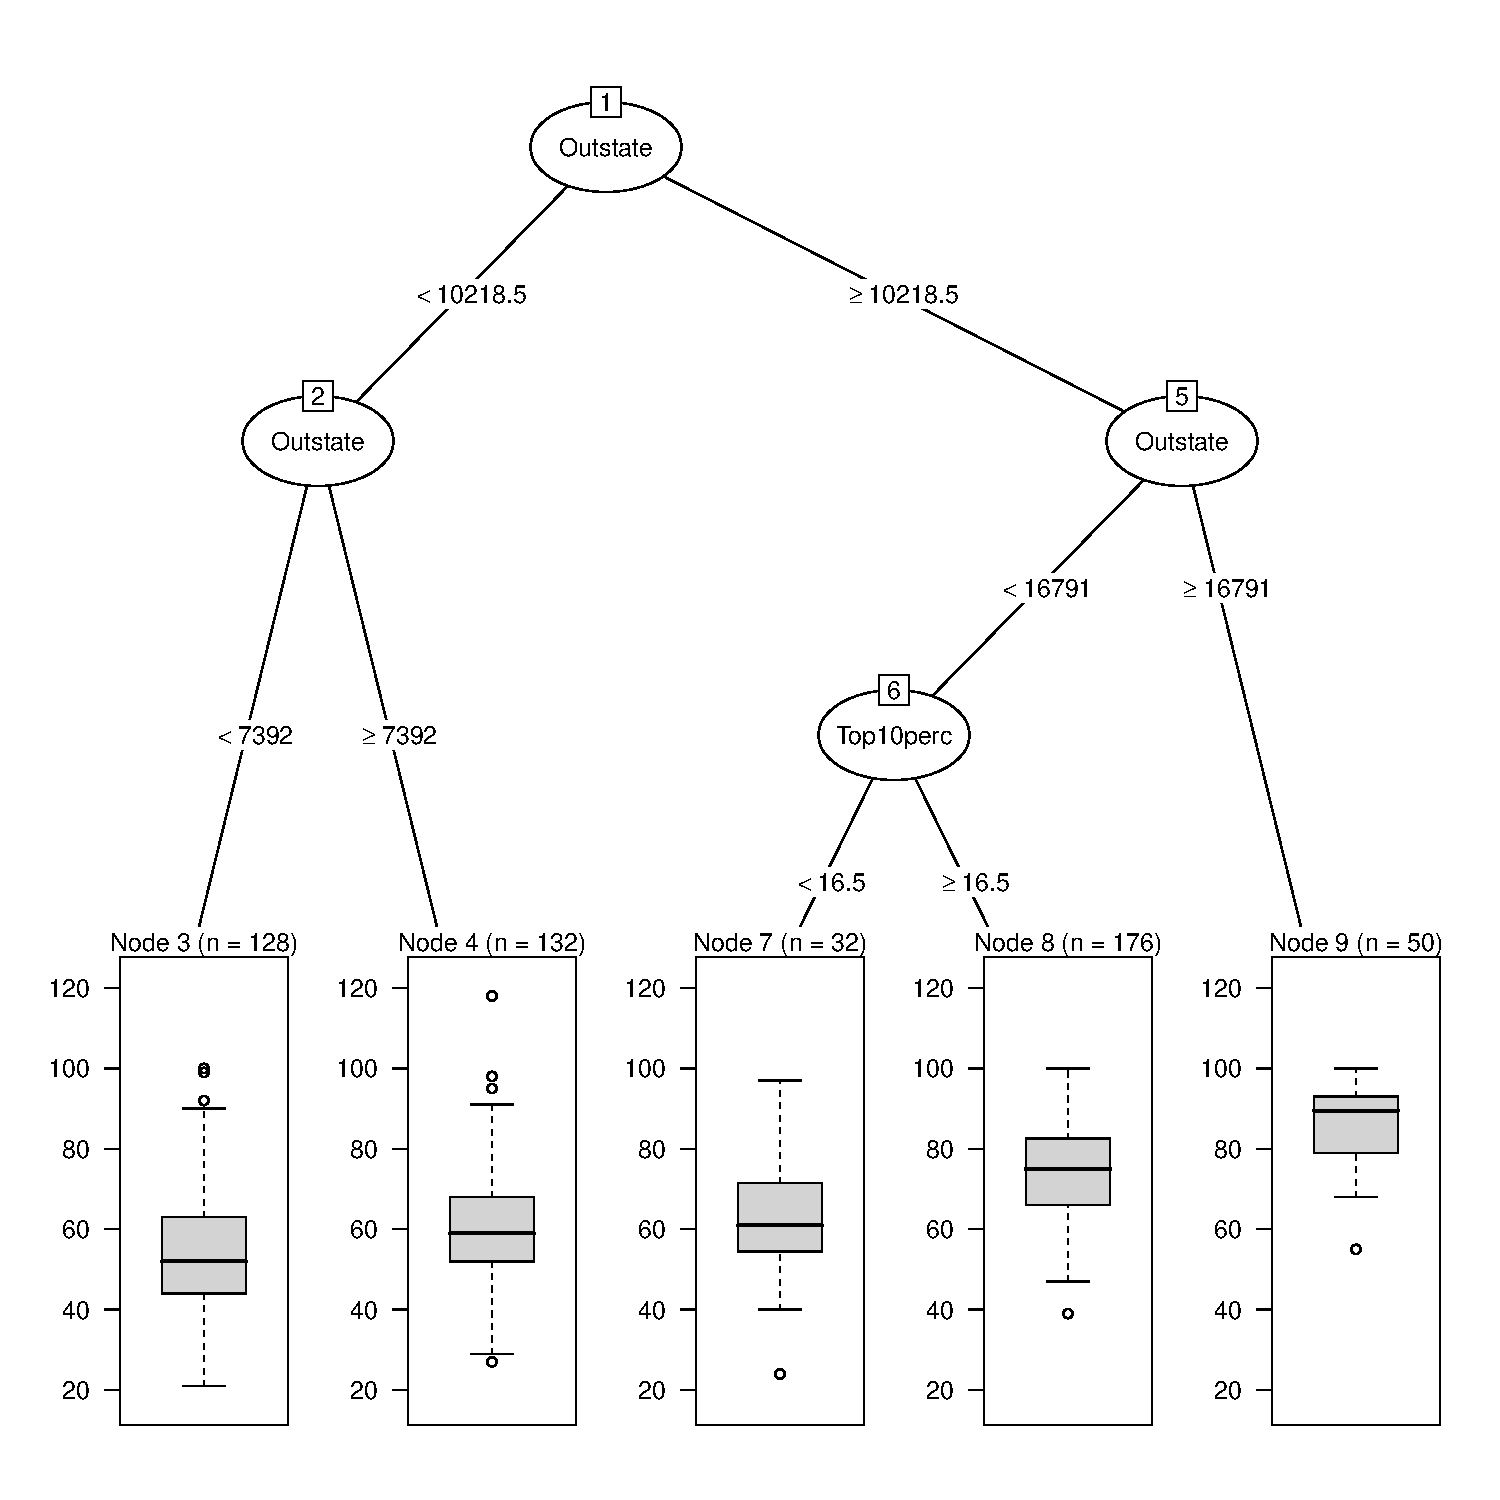
\includegraphics[width = 3.5in]{Figures/Chapter02/example_tree.pdf}} 
\end{tabular}
\caption[An example decision tree.]{\textit{(a) shows how college graduation rates vary as a function of out-of-state tuition and percentage of students in the top 10\% of their high school class. These partitions are created by a set of binary decision rules, shown in (b).}}
\label{fig:exampletree}
\end{figure}


%----------------------------------------------------------------------------------------

\subsection{Understanding the bias-variance tradeoff}


	In the previous example, we see the last split results in a subsection with a small sample size ($N = 32$). When growing a decision tree on an initial data set, referred to as the \textit{training set}, creating a tree with more depth and complexity will yield excellent performance. However, because of the subtleties in the data at hand, the same tree is likely to have poor performance generalizing to independent data. In other words, the tree algorithm is \textit{overfitting} the data. This highlights the importance of validating a decision tree (or any predictive model for that matter) on a separate data set, referred to as the \textit{test set}, to get a more accurate estimation of its generalizability.


	The underlying reason overfitting occurs is due to the \textit{bias-variance tradeoff}. Conceptually, bias refers to the difference between a true value and the average prediction of said value over many sample data sets drawn from the same population. Variance, on the other hand, refers to how much variability exists in your predictions for a given data point. Models of low complexity typically have high bias and lower variance, while models of high complexity typically have low bias and high variance. Overfitting occurs when your model has too much variance due to being overly complex, resulting in predictions that generalize poorly to new data \cite{hastie2009elements}. Thus, this bias-variance tradeoff is a balance between trying to identify a model with low bias that is still parsimonious enough to perform well on new data. Refer to \autoref{fig:tradeoff} to see how predictive performance varies as a function of model complexity between a training set and a test set in the graduation rate data. As the predictive model becomes more complex (i.e., more splits in the case of a decision tree), the estimated error always improves in the training set, but only improves to a certain extent in the test set. In this case, there is evidence for overfitting when the decision tree contains more than three or four splits. 


\begin{figure}[h]
  \centering
  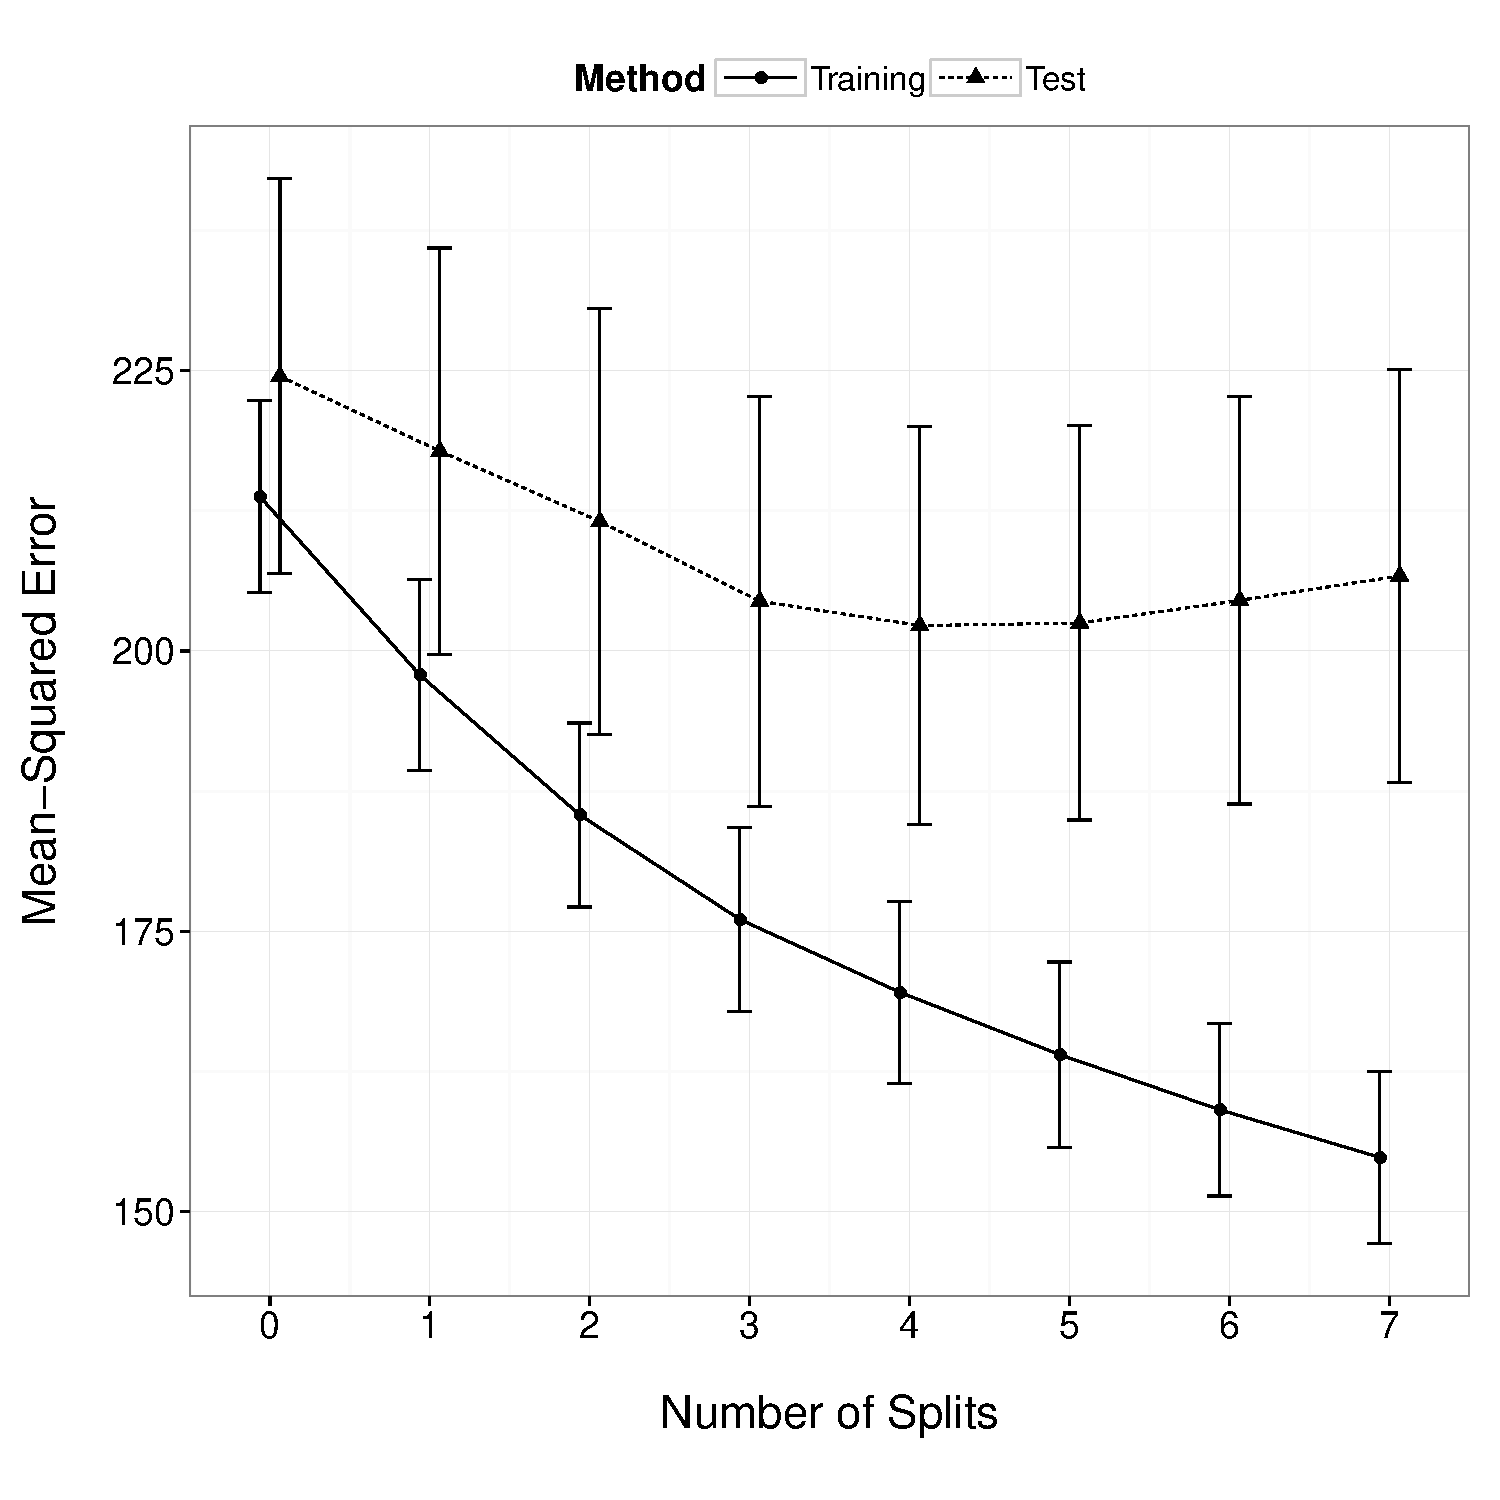
\includegraphics[width=3.5in]{Figures/Chapter02/bias_var_plot.pdf}
  \caption[The bias-variance tradeoff in the graduation rate data.]{\textit{The bias-variance tradeoff found in the graduate rate data, depicting how the error changes as a function of model complexity. The data was split into training and test sets 100 times to estimate precision, and the bars represent 1 standard error. Note that this figure was inspired by \cite{james2013introduction}.}}
  \label{fig:tradeoff}
\end{figure}


	The bias-variance tradeoff can also be understood mathematically as a decomposition of the residual term in a given statistical model. Given a training set consisting of data points $x_i, \ldots, x_n$, each with a corresponding $y_i$, we can assume there exists some true functional relationship, $y_i = f(x_i) + \epsilon$, where $\epsilon$ is a noise term with a mean of zero and variance $\sigma^2$. By choosing some statistical method, say linear regression, we get an estimate of $f(x)$, namely, $\hat{f}(x)$. The total squared error of this estimated function relation can then be defined as:

\begin{equation}
\begin{aligned}
\mathbb{E}[(y - \hat{f}(x))^2] &= \mathbb{E}[(f(x) - \mathbb{E}[\hat{f}(x)])^2] + \mathbb{E}[(\hat{f}(x) - \mathbb{E}[\hat{f}(x)])^2] + \mathbb{E}[\epsilon^2] \\
&= Bias(\hat{f}(x))^2 + Variance(\hat{f}(x)) + \sigma^2
\end{aligned}
\end{equation}


%----------------------------------------------------------------------------------------

\subsection{Pruning decision trees with cross-validation}


	Because decision trees that are too complex typically yield poor generalization performance, an additional step must be introduced into the process of building and evaluating a decision tree. How this issue is typically handled is with a procedure known as \textit{pruning}. That is, trees are initially grown out to their maximum depth (i.e., maximum complexity) with the algorithm outlined above. Then, the depth of the tree is reduced based on a given cost function. For any subtree $T$ that is a subset of a decision tree grown to full length, define $|T|$ as the number of terminal nodes in $T$, and $\alpha \geq 0$ as the complexity parameter. The updated cost-complexity measure, $RSS_{\alpha}(T)$, can be given as


\begin{equation}
RSS_{\alpha}(T) = RSS + \alpha|T|
\end{equation}


\noindent Here, the complexity parameter can be tuned to control how complex the resulting tree is. If $\alpha = 0$, no pruning will be done. When this value increases, however, the depth of the tree will get smaller. 

	The cost complexity parameter only has a finite number of values, because there is only a finite number of subtrees within a given tree. Once all the alpha values corresponding to unique subtrees have been collected, the value correponding to the best performance is selected with a procedure known as \textit{k-fold cross-validation}. This procedure first divides the training set into $K$ equal-size partitions, or folds. First, a full tree is grown on all but the $k$th fold. The mean squared error is then extracted from the left-out $k$th fold as a function of the complexity parameter. This procedure is repeated $K$ times, so every partition has an opportunity to act as a test set. The complexity parameter value that leads to the lowest average error across the $K$ estimates is chosen for the creation of the final tree to be used for future predictions. Note that setting $K$ as five or ten yields a good approximation to the true test error in many applications, so these values for $K$ are typically chosen \cite{hastie2009elements}. Another rule of thumb for selecting the value of the complexity parameter is known as the \textit{1-SE rule} \cite{breiman1984classification}. Because the cross-validation estimate of the complexity parameter results in a distribution of error estimates, the value of the complexity parameter is selected such that the simplest tree within one standard error of the best tree is chosen. 
	

	\autoref{fig:pruning} shows how the 1-SE rule is applied in practice for the college graduation rate data set. Recall that \autoref{fig:tradeoff} indicated that three or four splits should be made, while the 1-SE rule indicates only one split should be made. This highlights a feature of the 1-SE rule, in that it typically selects more parsimonious models, which may or may not yield better generalization performance. Thus, the result of the 1-SE rule should be compared with other evidence, like \autoref{fig:tradeoff}, to help determine how best to prune a decision tree. 


\begin{figure}[h]
  \centering
  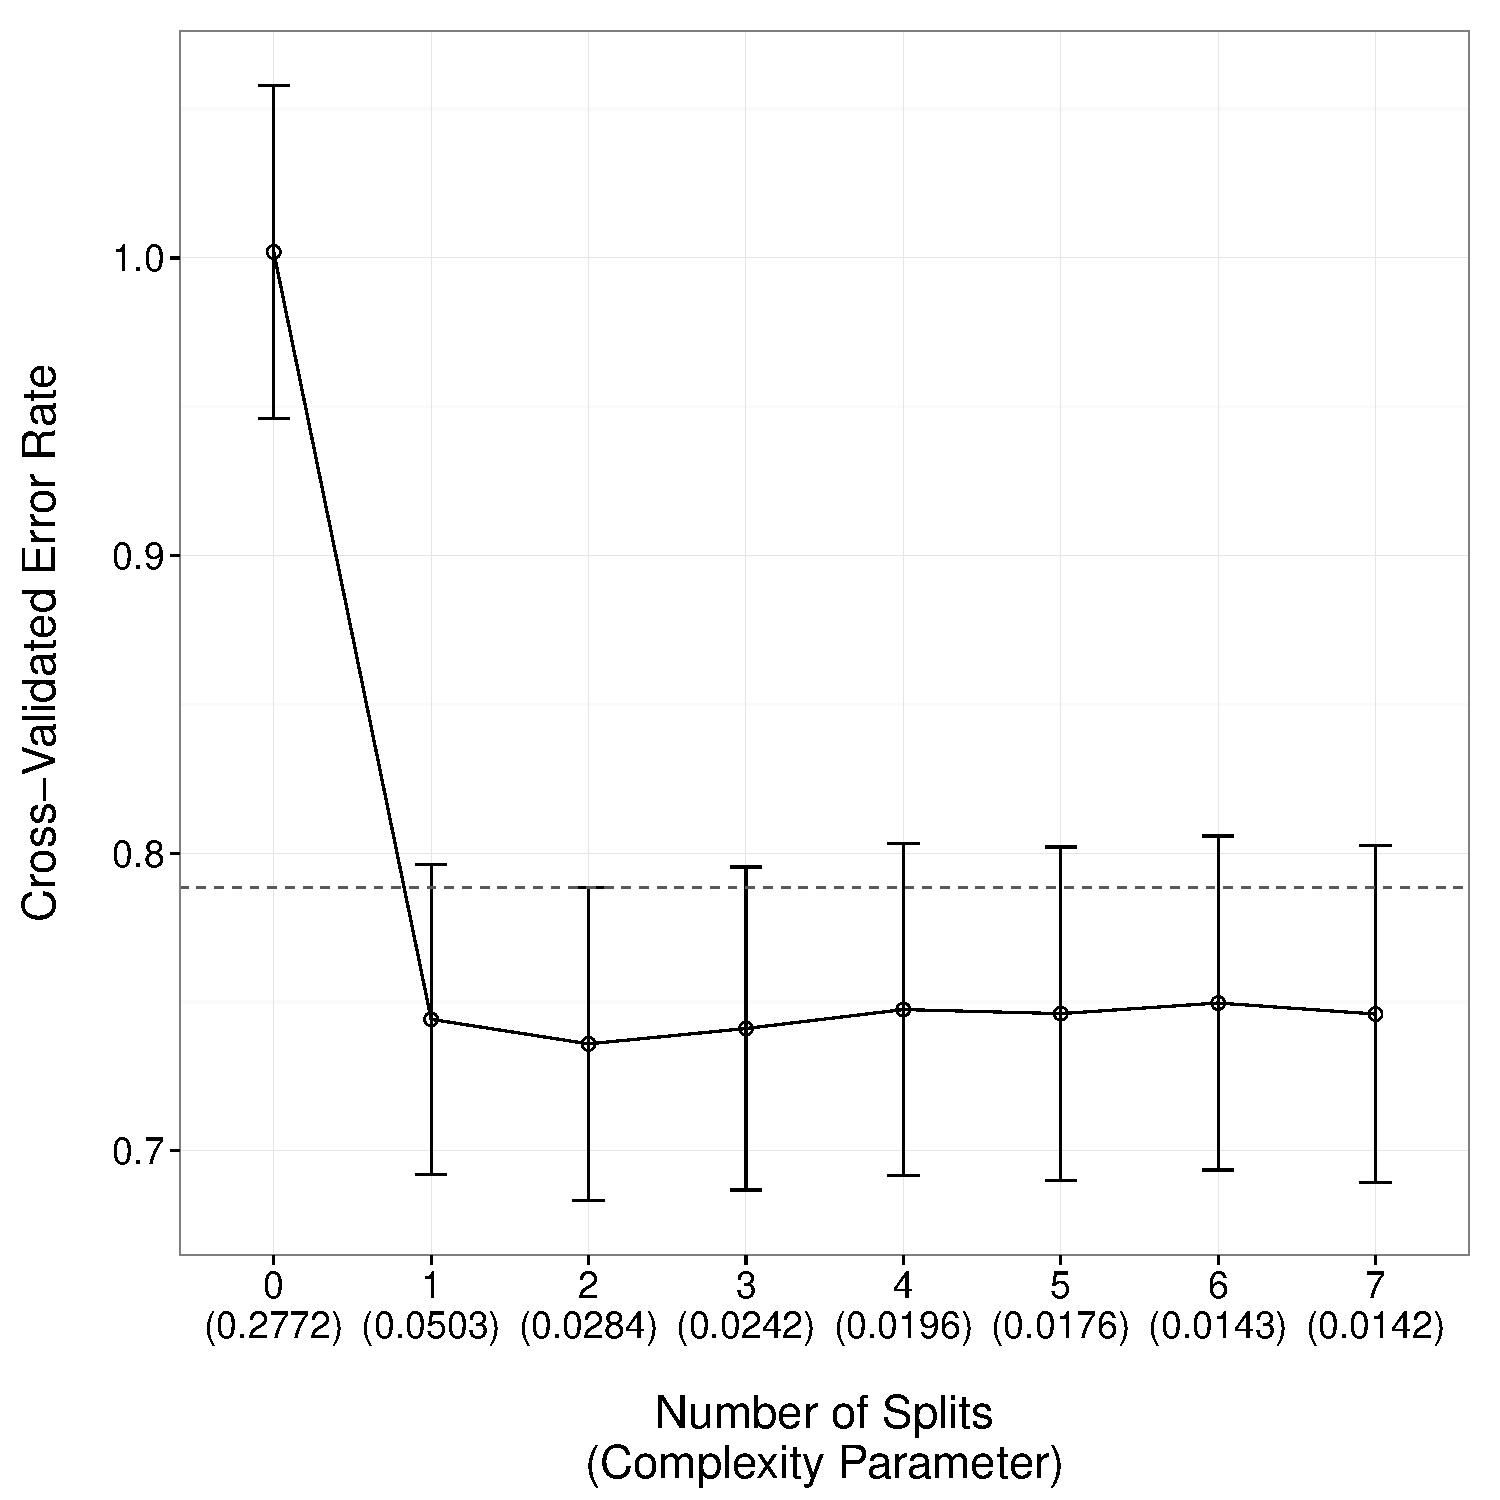
\includegraphics[width=3.5in]{Figures/Chapter02/cp_plot.pdf}
  \caption[Using cost-complexity pruning on the graduation rate data set.]{\textit{How the 10-fold cross-validation error changes as a function of model complexity in the college graduation rate data set. The 1-SE rule is set with the dotted line, indicating that this rule of thumb would select one split. Just selecting the tree that yields the minimum cross-validated error would select a tree with two splits.}}
  \label{fig:pruning}
\end{figure}


%----------------------------------------------------------------------------------------

\subsection{CART with a categorical outcome}

	While not discussed in the introduction to CART above, the algorithm can easily be extended to a categorical outcome with K potential classes by simply modifying the RSS criteria for both the splitting and pruning. More specifically, three methods exist as a measure of node purity in the case of a categorical outcome: classification error, the Gini index, and cross-entropy. Classification error is the simplest of the three, and is the fraction of observations in the training set that do not belong to the most common class


\begin{equation}
Classification \ error = 1 - \max_k(\hat{p}_{jk})
\end{equation}


\noindent where $\hat{p}_{jk}$ corresponds to the proportion of observations in the training set in the $j$th subsection that are from the $k$th class. While the classification error rate only includes the most common class, the Gini index reflects a measure of total variance across all possible classes


\begin{equation}
Gini = \sum_{k=1}^{K}\hat{p}_{jk}(1 - \hat{p}_{jk})
\end{equation}


\noindent Finally, cross-entropy is numerically similar to the Gini index, and is defined as


\begin{equation}
Entropy = -\sum_{k=1}^{K}\hat{p}_{jk}log(\hat{p}_{jk})
\end{equation}


	The relation between these three measures can be seen in \autoref{fig:compare_cat}. When the probability of belonging to a class in a given node becomes more certain (i.e., closer to 0 or 1), the values of all three measures get closer to zero. Otherwise, when the probability of an observation belonging to a specific class gets more uncertain (i.e., closer to 0.5), the value of these measures increase. In other words, these measures calculate how homogenous a given node is, and the goal of the recursive partitioning algorithm is to minimize this value over all nodes in the splitting process. Note that either the Gini index or cross-entropy are typically favored in the splitting process, as they are more sensitive to node purity when compared with the misclassification rate \cite{james2013introduction}. If the probabilities of a given class are small, cross-entropy is likely a better choice compared with the Gini index, because of the log in the calculation. However, research has found no conclusive evidence regarding whether the Gini index or cross-entropy yields better performance in a general sense \cite{raileanu2004theoretical}.


\begin{figure}[h]
  \centering
  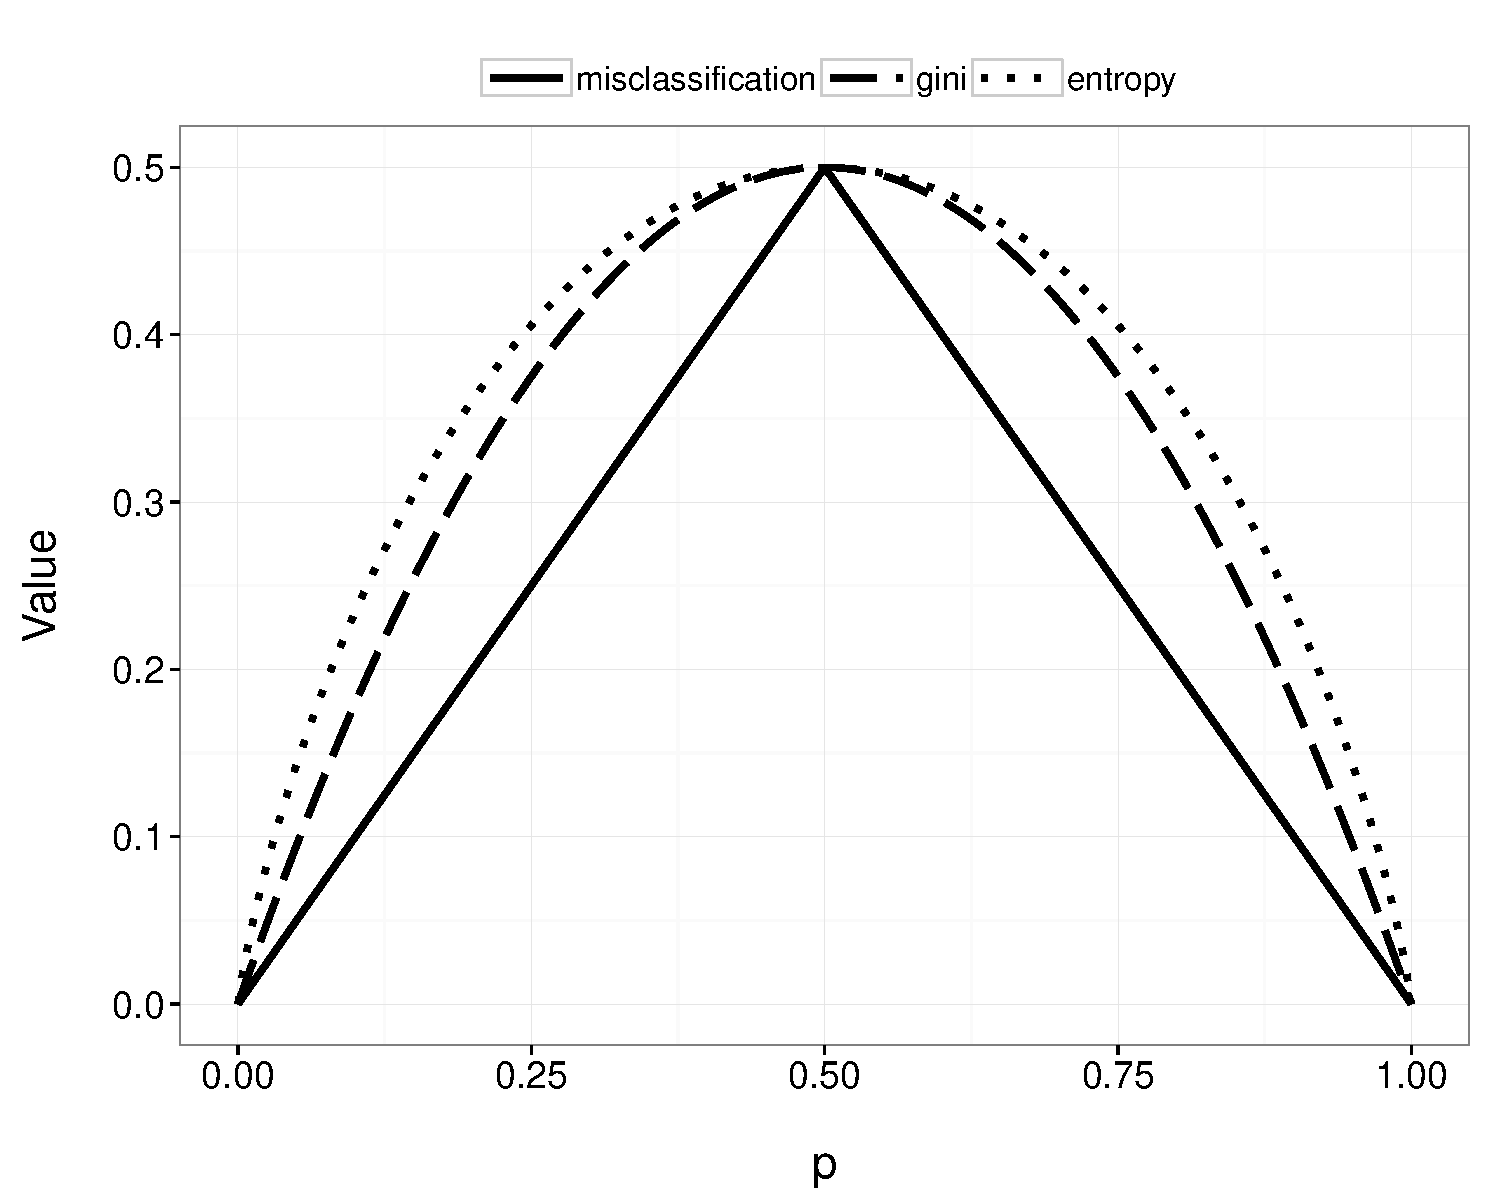
\includegraphics[width=3.5in]{Figures/Chapter02/compare_cat_long.pdf}
  \caption[The relation between classification error, the Gini index, and cross-entropy.]{\textit{The relation between classification error, the Gini index, and cross-entropy at different probability values for belonging to a given class when two classes are present. Image adapted from \cite{hastie2009elements}.}}
  \label{fig:compare_cat}
\end{figure}



%----------------------------------------------------------------------------------------

\subsection{Pros and cons of CART}


	CART is a method that can efficiently search a parameter space, capturing potential non-linear relations as well as higher-order interactions without explicit model specification by the researcher. It can also handle both continuous or categorical variables as outcomes by simply changing the underlying measure of node purity. Finally, and perhaps the most relevant to this dissertation, is that the resulting pruned tree is fairly easy to understand and explain to others, even if those individuals are not familiar with the technique or lack a formal statistical background.


	Despite all these advantages, CART is not without drawbacks. First, like all simple decision trees, they generally do not yield good predictive performance when compared to other regression-based techniques \cite{james2013introduction}. Pruning can also add a layer of researcher subjectivity in deciding how complex or simple a given tree is. Finally, because the splitting procedure considers all possible splits within all possible variables simultaneously, variables with more potential splits are more likely to be chosen to have a potential split point purely due to chance when compared with variables with less potential splits \cite{loh1997split, quinlan1995oversearching}. For example, there are $N - 1$ potential splits for a continuous variable (assuming no identical values among observations) and $2^{K - 1} - 1$ potential splits for categorical variables with $K$ categories. Assuming a sample size of 100, a continuous variable with no repetitive numbers or a categorical variable with five classes will have 99 and 624 potential splits respectively, while a 5-point Likert scale item or a dichotomous variable will have substantially less (4 and 1, respectively).


%----------------------------------------------------------------------------------------

\section{Conditional inference trees}


	To mitigate the issue of pruning and the biased splitting procedure found in many recursive partitioning algorithms, \citeA{hothorn2006unbiased} proposed conditional inference trees (CTREE). While conceptually similar to CART, CTREE is based on a well-defined theory of permutation tests developed by \citeA{strasser1999asymptotic}. Like CART, CTREE also consists of four main steps, which will first be explained conceptually. First, a global null hypothesis of independence between $Y$ and all covariates $X_j$ is tested. For a common example, if all covariates and the outcome are continuous, a Pearson's correlation coefficient with a corresponding p-value is calculated for each variable's association with the outcome. If no p-value is below the pre-selected alpha level after accounting for multiple significance tests, the global null hypothesis is not rejected and the algorithm terminates. Otherwise, the covariate with the stongest association (i.e., p-value) with the outcome is selected for splitting. The best split within this covariate is selected, and the training set is partitioned on this value. Finally, these steps are iteratively repeated until the global null hypothesis can no longer be rejected in all subsections. 

	These four steps can also be explained mathematically following notation from \citeA{hothorn2006unbiased} and \citeA{molnar2013}. 

\vspace{8ex}

\noindent Step 1: The Global Null Hypothesis Test \\

First, in a given sample, assume there exists a response $Y$ and a covariate vector $X = (X_1, \ldots, X_p)$. Let $D(Y|X)$ represent the conditional distribution of response $Y$ given the covariates $X$, and $L_n$ represent the training set, such that $L_n = [Y, X_1, \ldots, X_p]$. The global null hypothesis is then defined as $H_0 = \bigcap_{j=1}^{p}H_0^j$, where $H_0^j: D(Y|X_j) = D(Y)$. This is tested with the following test statistic. 


Let $g_j$ be a transformation of the covariate $X_j$, such that $g_j:X_j \rightarrow \mathbb{R}^{p_j}$, where $p_j$ is the number of dimensions the covariate $X_j$ is transormed into. The \textit{influence function}, $h$, performs a similar transformation on the outcome, such that $h: y \rightarrow \mathbb{R}^q$. Also, let $w$ correspond to a set of weights indicating whether a given observation is in a node or not (i.e., set at 1 or 0). The test statistic for every covariate $j$ can be defined as\footnote{Note that this notation differs slightly from \citeA{hothorn2006unbiased}, where $h(Y_i)$ is written as $h(Y_i, (Y_1, \ldots, Y_n))^T$. This was removed for simplicity.}

\begin{equation}
\label{eq:teststat}
T_j(L_n, w) = vec\left ( \sum_{i=1}^{n}w_ig_j(X_{j,i})h(Y_i)^T \right ) \in \mathbb{R}^{p_jq}
\end{equation}


\noindent where the resulting $p_j \times q$ matrix is converted into a $p_jq$ column vector using the $vec$ operator. Note that this final conversion is not a necessity, but is done for computational simplicity. 


 Both the transformation and influence function are chosen depending on the scales of $X_j$ and $Y$, respectively. An outline for selecting both $g$ and $h$ can be found in \citeA{hothorn2006unbiased}. In the frequent case of a numeric variable for both covariate and outcome, both functions can be the identity, indicating that no transformation is made. In the case of a categorical variable, the transformation for said variable can map the covariate into a variable with the number of dimensions equal to the number of categories (i.e., two dimensions in the binary case, with $(1, 0)^T$ for one condition and $(0, 1)^T$ for the other). 


Because the distribution of $T_j$ under the null hypothesis is unknown for most instances, it must be estimated via a \textit{permutation test} framework. That is, a null distribution is contructed by fixing the covariate values and permuting the outcome to destroy the relationship between the covariates and the outcome. The derivation of the conditional expectation $\mu_j$ and covariance $\Sigma_j$ under the null can be found in \citeA{hothorn2006unbiased}, and are not included here for brevity.

With the conditional expectation and covariance, $T \in \mathbb{R}^{pq}$ can be standardized. Let $t$ be the value of $T$, $\mu$ be the expected value of $T$ and $\Sigma_{kk}$ is the $k$th diagonal entry of the covariance matrix under the null distribution. Using these, the maximal entry of $T$ after standardization is chosen for a test statistic $c$:

\begin{equation}
\label{eq:stdteststat}
c(t, \mu, \Sigma) = \max_{k=1,\ldots, pq}\left | \frac{(t - \mu)_k}{\sqrt{\Sigma_{kk}}}  \right |
\end{equation}


The test statistic for each variable, $c(T_j(L_n, w), \mu_j, \Sigma_j)$, is then converted to a p-value scale in order to test the global null hypothesis and for the purpose of variable selection. To reiterate the most recent steps incorporating the permutation test, all observations in a given subsection are randomly permuted, and $c$ is calculated for each covariate. The resulting permuted distribution for a given variable then corresponds to the null distribution assuming no relationship between that variable and the outcome, and a p-value can be calculated as the proportion of the null test statistic distribution that is larger in magnitude than the observed test statistic. The p-values for each variable are corrected for a global test using a multiple comparisons procedure (e.g., Bonferroni), and then compared to the preset $\alpha$ level which is typically (and arbitrarily) defined to be 0.05. If the global test is not rejected, the algorithm makes this node a terminal node. 

\vspace{2ex}

\noindent Step 2: Variable Selection \\


If the global test is rejected, then the variable with the lowest p-value calculated in Step 1 is selected for splitting.

\vspace{3ex}

\noindent Step 3: Split Point Selection \\

Once the variable has been selected, splits are determined using a special case of the test statistic formula defined in \autoref{eq:teststat}. For a selected variable, $X_j*$, the equation is 

\begin{equation}
T_{j*}^A(L_n, w) = vec\left ( \sum_{i=1}^{n}w_iI(X_{j*,i} \in A)h(Y_i)^T \right ) \in \mathbb{R}^q
\end{equation}

\noindent where A is a possible partition of the current observations and

\begin{equation}
I(X_{j,i} \in A) = \left\{
     \begin{array}{rr}
       1 & : X_{j,i} \in A \\
       -1 & : X_{j,i} \notin A
     \end{array}
   \right.
\end{equation}

Note that the values are coded as 1 and -1 so if a given covariate is independent of the outcome, the corresponding values will typically cancel and yield a value for $T_{j*}^A$ that is close to zero.

As defined, this sequence will test all possible subsets of $A$. To reduce the amount of computation, possible subsets for continuous and ordinal variables are restricted to maintain their order among observations. An additional contraint can be made by requiring a minimum node size for all groups within a given subset. Finally, a partition, $A^*$, is identified as the one which maximizes the standardized test statistic using \autoref{eq:stdteststat} with the proposed new split $A$. That is,

\begin{equation}
A^* = \underset{A}{\operatorname{argmax}} \ c(t_{j*}^A, \mu_{j*}^A, \Sigma_{j*}^A)
\end{equation}

\vspace{1ex}

\noindent Step 4: Repeat \\

The weights within each node are re-normalized, and these steps are repeated until the global null hypothesis is no longer rejected in each subsection.


\vspace{2ex}


Clearly, this algorithm is very similar to CART in its basic iterative partitioning structure. Similarly, conditional inference trees can be pruned by altering the significance level required in the splitting process, which can be estimated via a cross-validation procedure \cite{hothorn2006unbiased}. Refer to \autoref{fig:comparetree} for a visual comparison between the final CTREE and CART models using the graduation rate. These two methods often yield similar predictive performance despite having different tree structures.


\begin{figure}
\begin{tabular}{c}
\subfloat[]{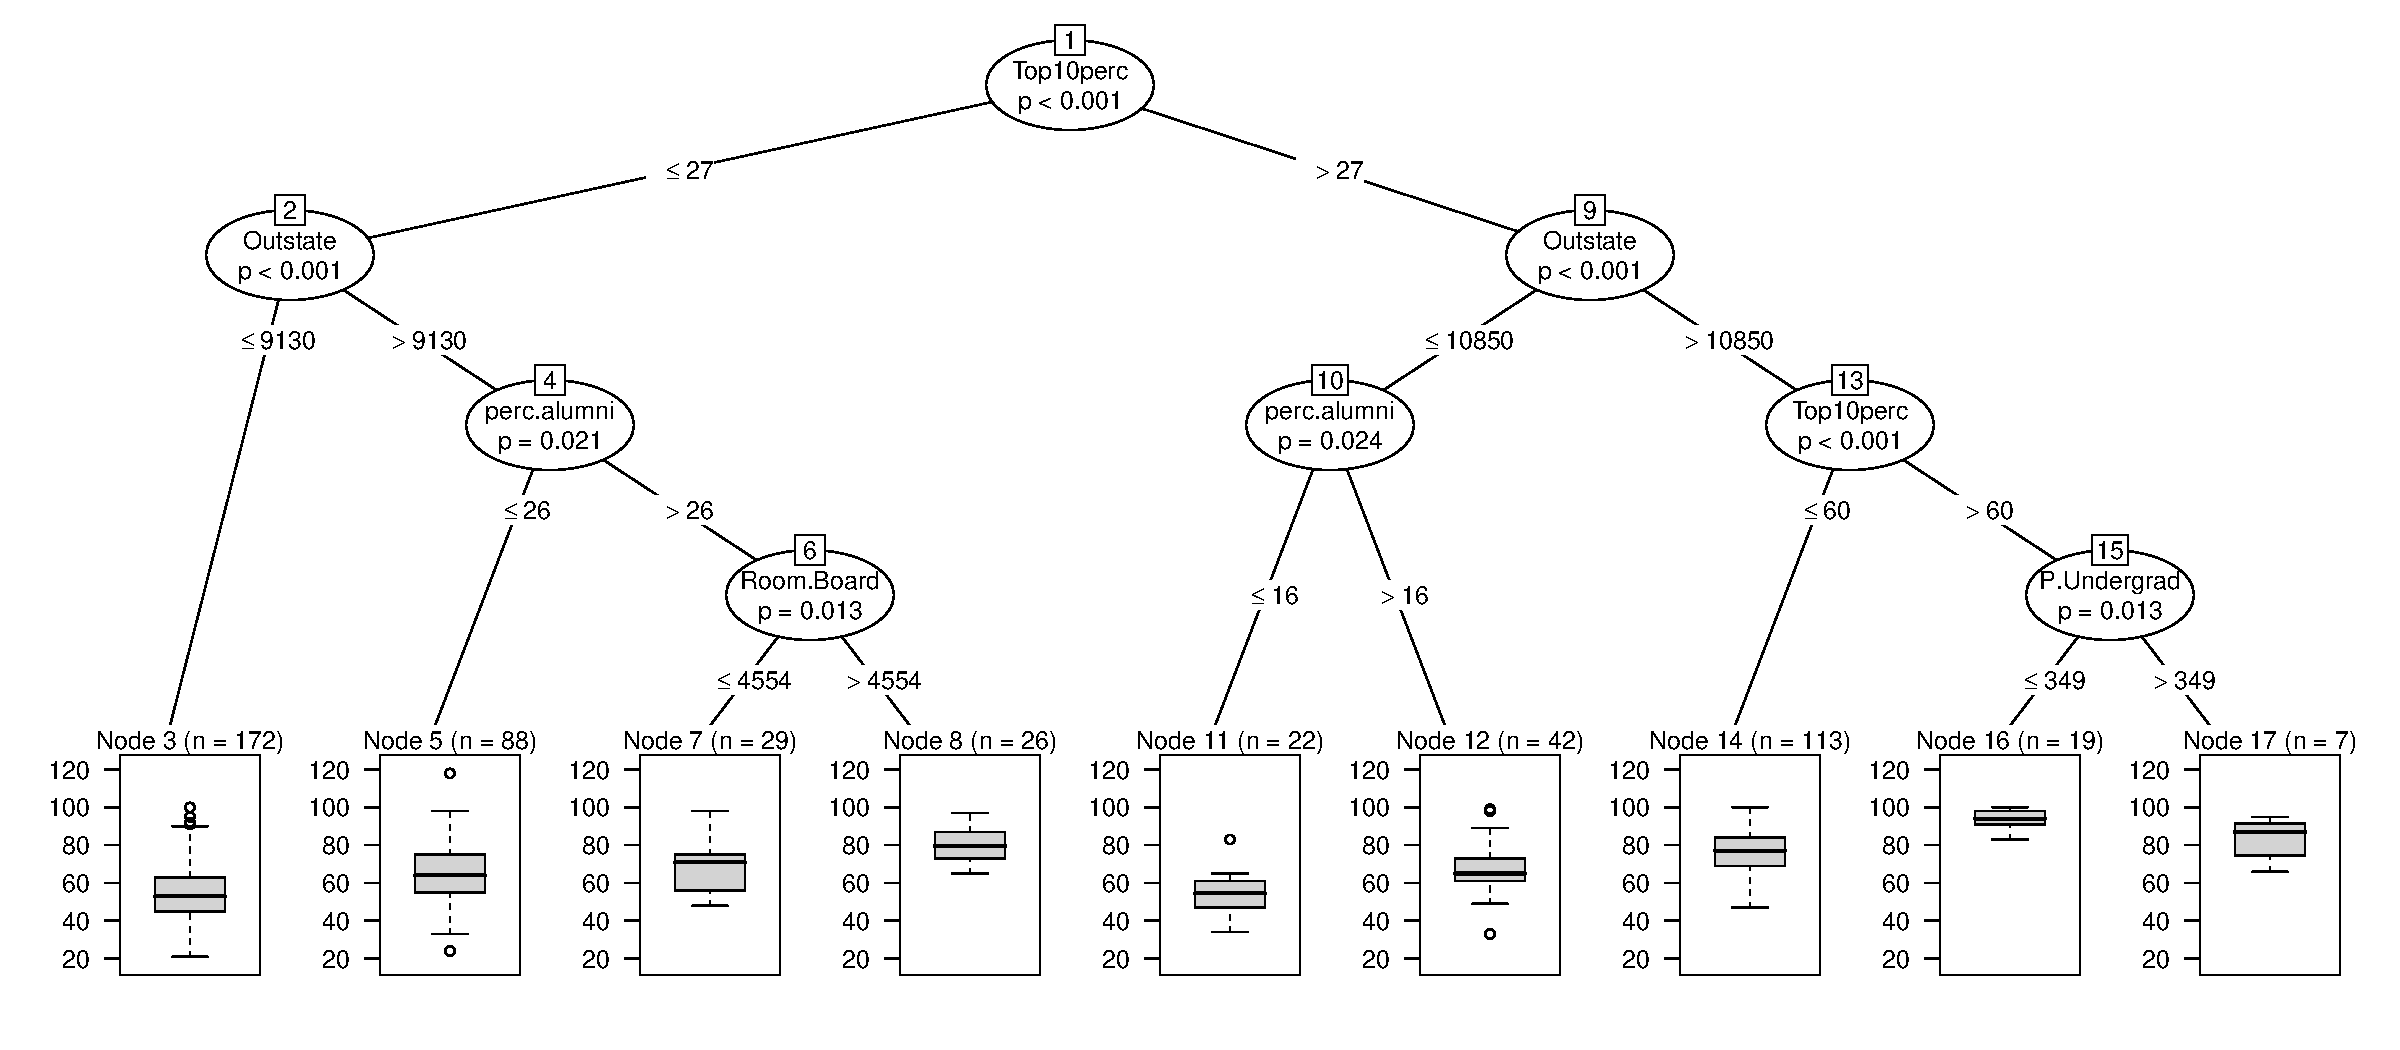
\includegraphics[width = 4.5in]{Figures/Chapter02/ci_tree.pdf}} \\
\subfloat[]{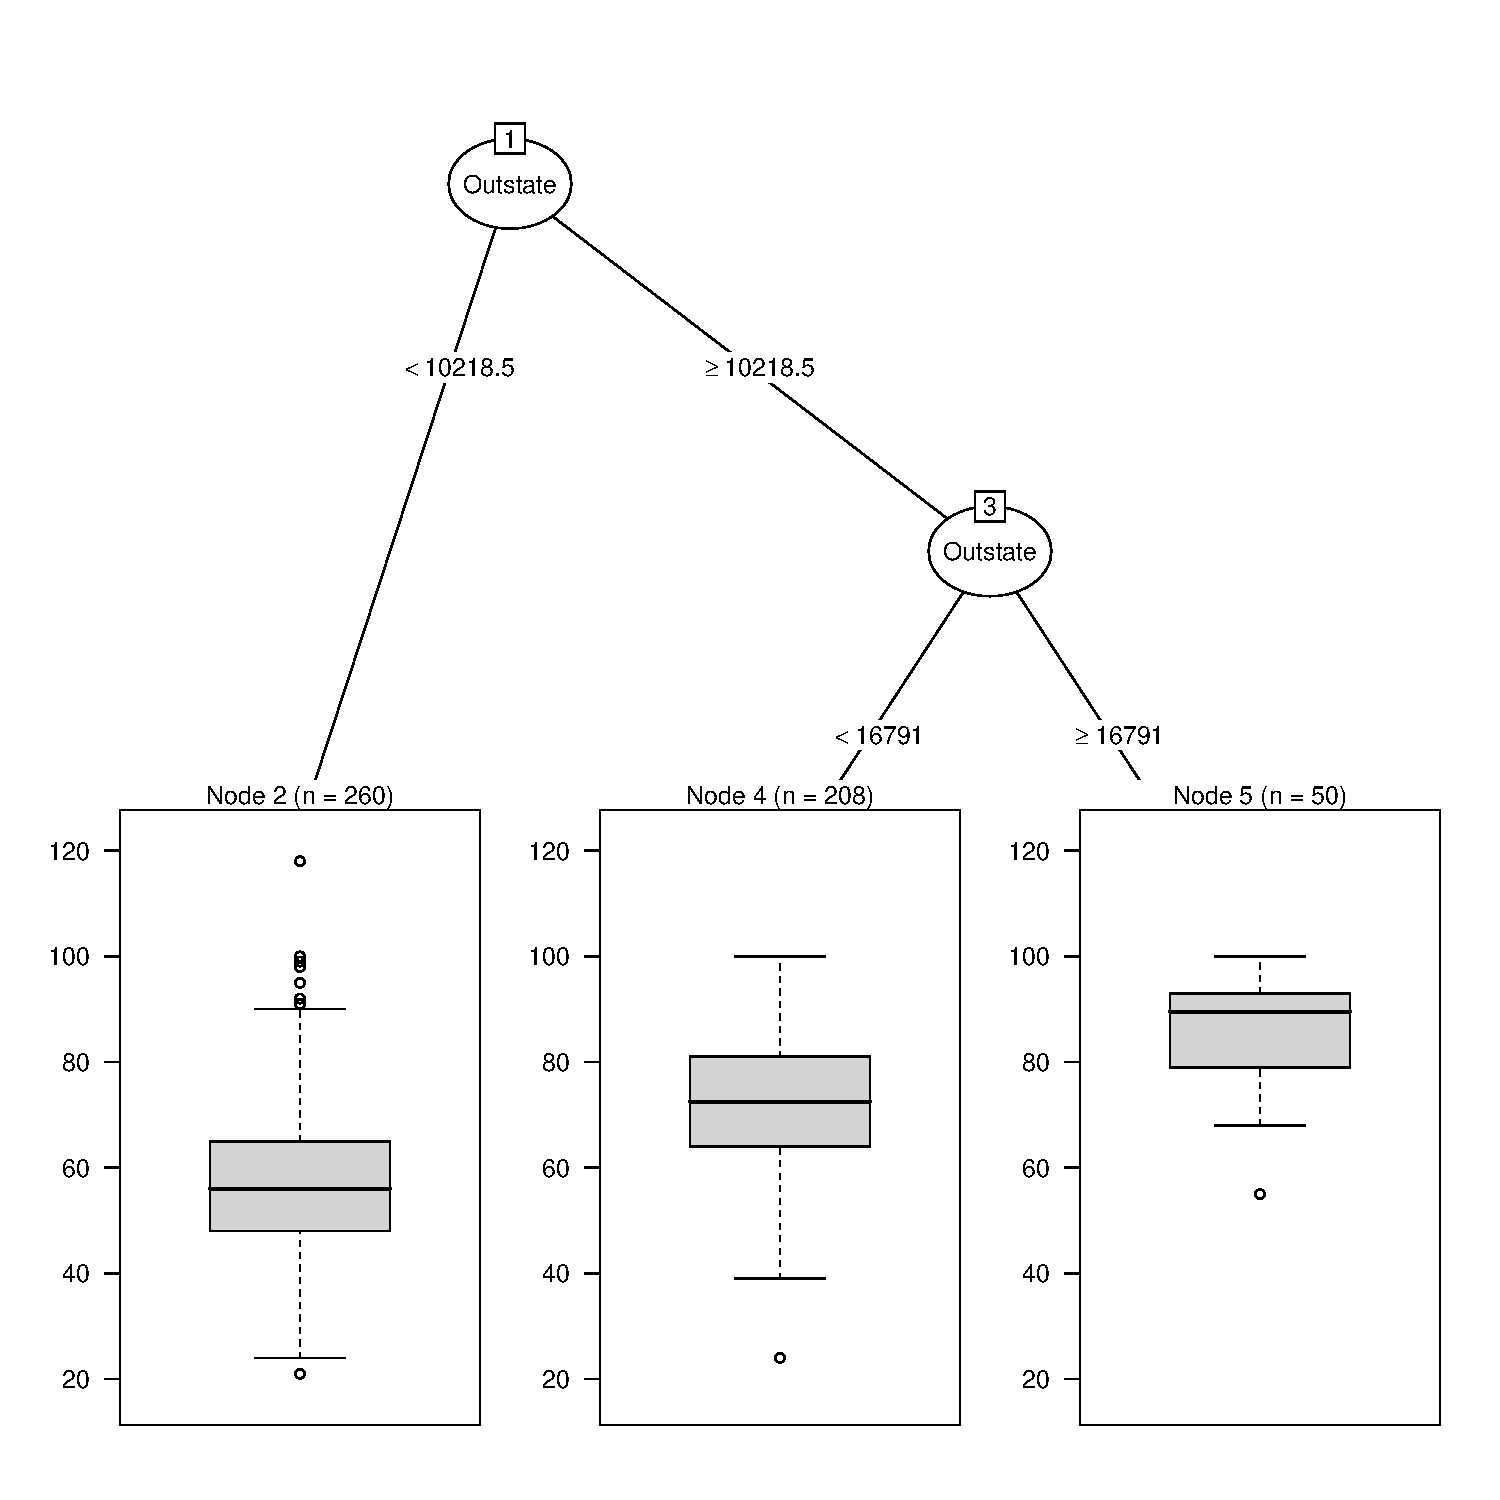
\includegraphics[width = 4.5in]{Figures/Chapter02/cart_tree.pdf}} 
\end{tabular}
\caption[A comparison of a conditional inference tree and a pruned CART tree.]{\textit{A comparison of a conditional inference tree (a) and a pruned CART tree (b). Note that the conditional inference tree contains p-values refering to the significance of each split. Despite a different tree structure, both trees yield similar predictive performance.}}
\label{fig:comparetree}
\end{figure}



%----------------------------------------------------------------------------------------

\subsection{Pros and cons of conditional inference trees}


	Conditional inference trees house all the benefits of decision trees while simultaneously alleviating the issues of both pruning and biased variable selection found in CART. And yet, despite this lack of bias in the splitting procedure, CTREE and CART typically perform similarly with regard to predictive accuracy \cite{hothorn2006unbiased, strobl2007bias}. One downside to this method is that, because it incorporates a permutation framework, the algorithm is much more computationally expensive compared to CART. Thus, if the goal is to simply achieve good predictive accuracy in a tree framework, CART is typically a much better choice. Another major con with the conditional inference framework is that it assumes the data adhere to the traditional assumptions of independence. This potential issue with regard to multilevel data will be discussed further in \autoref{ch:problem}. Finally, like all decision trees, CTREE is a predictive method that is often outperformed by regression techniques. There are two main reasons for this. First, trees are predictive methods that possess high variance. Oftentimes, a small shift in the training set (e.g., sampling the training set more than once) will result in a completely different tree structure being detected \cite{hastie2009elements}. Second, smooth relationships often naturally occur in data sets, and can be better captured with the underlying additive structure found in regression methods compared to the binary, piecewise splits underlying decision trees.


%----------------------------------------------------------------------------------------

\section{Random Forests}


	As mentioned previously, while trees provide intuitive split criteria for a given data set, these decision rules suffer in generalizability performance due to having high variance. \citeA{breiman1996bagging} proposed a solution to this issue by repeatedly taking a bootstrap sample of the training set to create many decision trees, and then aggregating the results of all the trees together to create the final predictions. This technique, referred to as \textit{bagging} (short for bootstrap aggregating), led to better predictive performance due to the fact that trees grown to full length are predictors that have low bias and high variance. Essentially, by aggregating their predictions into an ensemble, this new method maintains the low bias found in single decision trees, but also has reduced variance by replacing the hard, piecewise fits found in decision trees with smoothed relations \cite{breiman1996bagging, buhlmann2002analyzing, strobl2009introduction}.

	One more improvement to this idea was made by \citeA{breiman2001random}. Due to the greediness of the recursive partitioning algorithm, a bagged ensemble of trees is typically dominated by one or two variables that are always used in the first split. This ignores the possibility of the existence of a tree with better predictive performance that contains a first split that is suboptimal. To give these lesser predictors a better chance to be incorporated into the splitting procedure, \citeA{breiman2001random} introduced \textit{random forests}, which first grew decision trees using a random subset of possible predictor values, and then used bootstrap aggregation to create an ensemble. In this method, both the number of variables to select for each tree and the number of trees to grow in total are parameters that can be tuned to yield better predictions. Many statistical software packages have sensible defaults for these values that typically yield good performance, suggesting that a random forest is a good ``off-the-shelf'' method that does not require as much tuning when compared to other predictive models \cite{strobl2009introduction}.


%----------------------------------------------------------------------------------------

\subsection{Out-of-bag samples}


	In a bootstrap sample, the probability of an observation being selected is $1 - (1 - \frac{1}{n})^n$. As $n \rightarrow \infty$, this value converges to approximately 0.632. Thus, by nature of the bootstrap process, approximately 63\% of the data set will be used for training in each decision tree. This highlights a nice feature of random forests, in that about 37\% of the data, referred to as the out-of-bag (OOB) sample, are not used in any given tree. Using the OOB samples to evaluate performance has been shown to be a good approximation of the error found in a separate test set \cite{hastie2009elements}, and are typically used as a replacement for the cross-validation step found in decision trees.


%----------------------------------------------------------------------------------------

\subsection{Variable importance}


	Because random forests include many trees, each with their own distinct set of decision rules, they inevitably become harder to interpret. However, both numerical and graphical methods do exist. One such method is known as \textit{variable importance}, and is typically measured in a permutation framework. More specifically, once an ensemble method has been created, the OOB samples are used to estimate predictive performance. Then, the same data is permuted with respect to a given variable in order to break that variable's link with the outcome, and the predictive accuracy of the overall forest is measured again. Finally, variables are assigned a value that corresponds to the difference in the original prediction accuracy and the permuted prediction accuracy. If the difference is large, then this indicates that the particular variable plays a more important role in predicting the outcome. Otherwise, if the predictive accuracy does not change very much, then this variable does not play a large role in predicting the outcome. See \autoref{fig:varimp} for the variable importance plot for the college graduation rate example. This plot confirms what was found in the single decision tree: out-of-state tuition is the most important variable for predicting college graduation rate.


\begin{figure}[h]
  \centering
  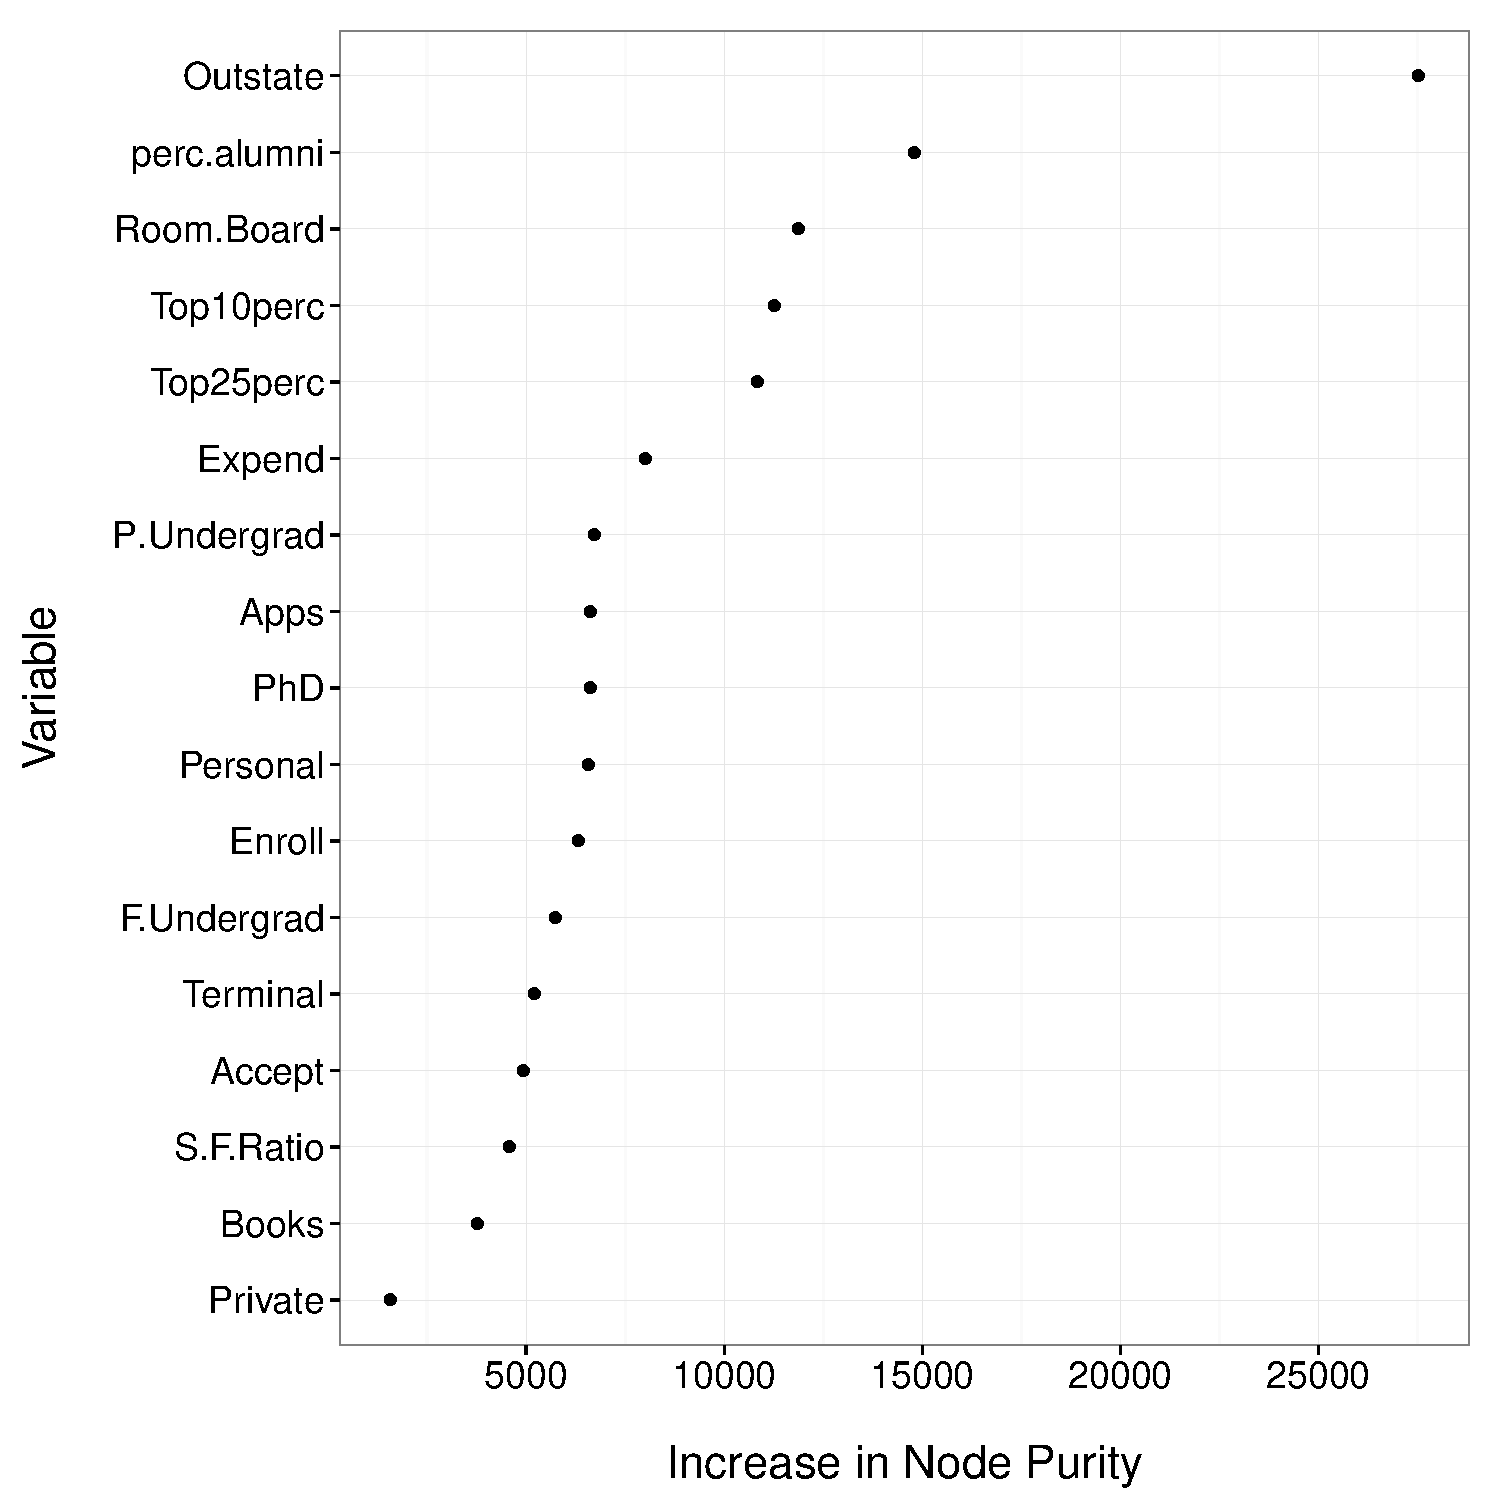
\includegraphics[width=3.5in]{Figures/Chapter02/var_imp_plot.pdf}
  \caption[Variable importance for a CART random forest.]{\textit{Variable importance for a CART random forest, indicating the out-of-state tuition has the largest role in predicting graduation rate.}}
  \label{fig:varimp}
\end{figure}


%----------------------------------------------------------------------------------------

\subsection{Partial dependence plots}


	While variable importance metrics are useful, the functional relations between the variables and the outcome remain hidden from view. One way to further investigate these relations is with \textit{partial dependence plots}. These plots are graphical visualizations of the marginal effect of a given variable (or multiple variables) on an outcome. Typically, these are restricted to only one or two variables due to the limits of human perception, and thus may be misleading due to hidden higher-order interactions. Despite this, partial dependence plots can still be extremely useful for knowledge discovery in large data sets, especially when the random forest is dominated by lower-order interactions and main effects. 


	Following the notation of \citeA{hastie2009elements}, partial dependence plots can be mathematically defined as follows. Suppose $S$ is a subset of $p$ predictor variables, such that $S \subset \left\{X_1, X_2, \ldots, X_p\right\}$. Let $C$ be a complement to $S$, such that $S \cup C = \left\{X_1, X_2, \ldots, X_p\right\}$. The random forest predictor function, $f(X)$, will depend upon all $p$ predictor variables. Thus, $f(X) = f(X_S, X_C)$. The partial dependence of the $S$ predictors on the predictive function $f(X)$ is


\begin{equation}
f_S(X_S) = \mathbb{E}_{X_C}[f(X_S, X_C)]
\end{equation}


\noindent and can be estimated by


\begin{equation}
\bar{f}_S(X_S) = \frac{1}{N}\sum_{i = 1}^{N}[f(X_S, X_{Ci})]
\end{equation}


\noindent where $\left\{x_{C1}, x_{C2}, \ldots, x_{CN}\right\}$ are the values of $X_C$ ocurring over all observations in the training data. In other words, in order to calculate the partial dependence of a given variable (or variables), the entire training set must be utilized for every set of joint values in $X_S$. As one can image, this can be quite computationally expensive when the data set becomes large. See \autoref{fig:partial_dependence} for examples of partial dependence plots for the college graduation rate data set. 

\begin{figure}
\begin{tabular}{c}
\subfloat[]{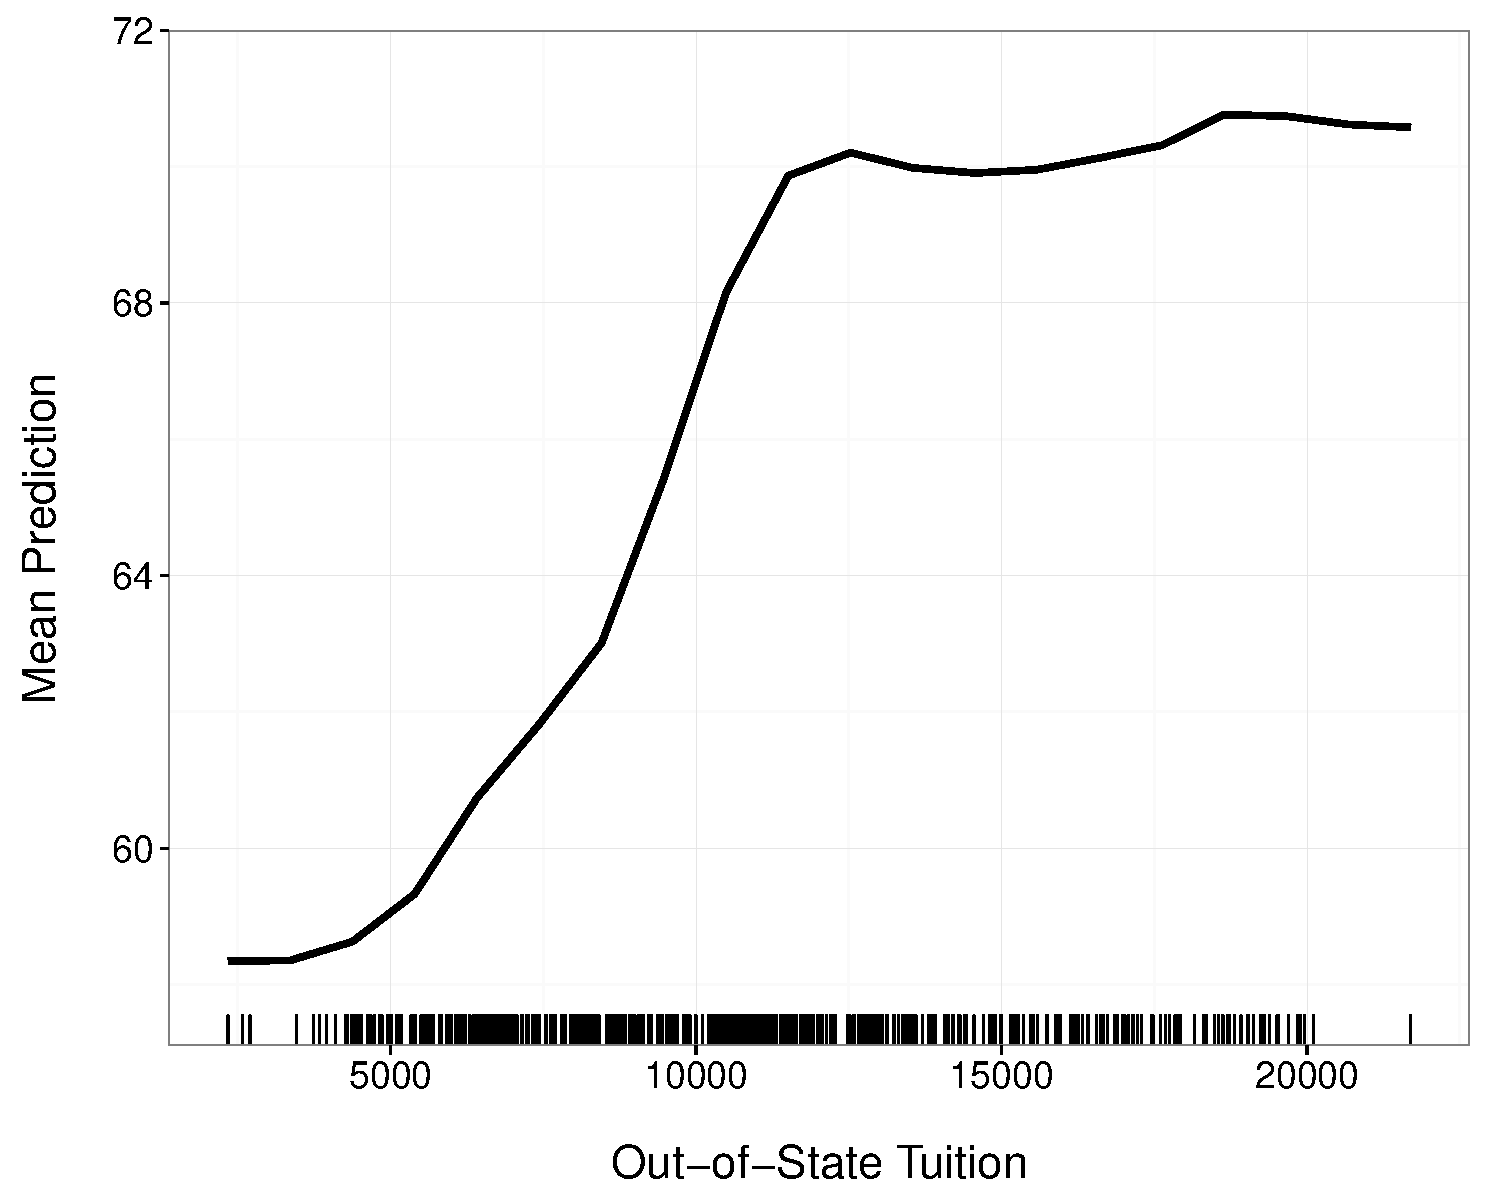
\includegraphics[width = 3.5in]{Figures/Chapter02/part_dep_Outstate.pdf}} \\
\subfloat[]{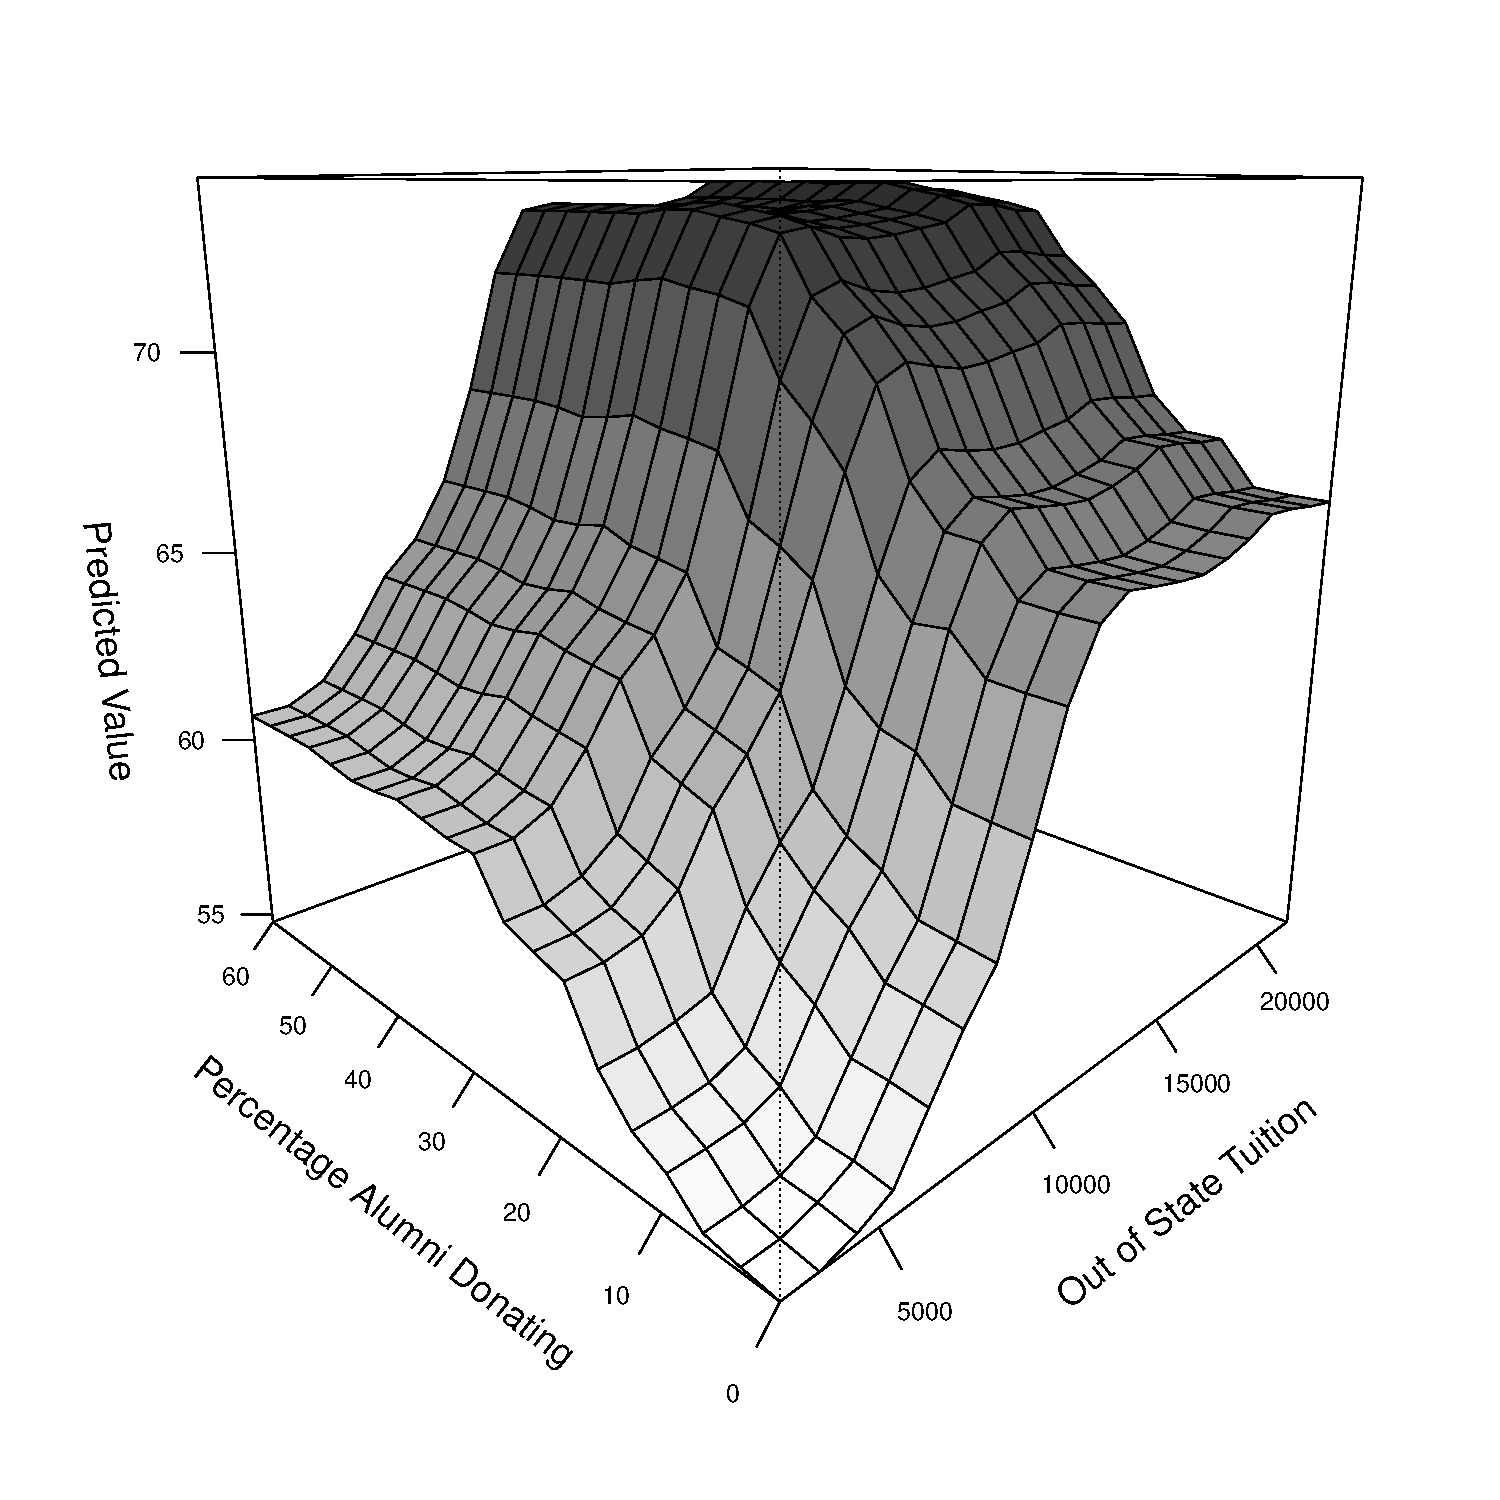
\includegraphics[width = 3.5in]{Figures/Chapter02/plot_3d.pdf}} 
\end{tabular}
\caption[Partial dependence plots for the graduation rate data.]{\textit{(a) shows the partial dependence plot for out-of-state tuition, revealing a somewhat linear relation with graduation rate. (b) shows the partial dependence plot between both out-of-state tuition and percent of alumni donating to the institution, resulting in a three-dimensional plot. Note that because both variables have consistent relations with graduation rate across the values of the other variable, there is no substantial evidence for a potential interaction.}}
\label{fig:partial_dependence}
\end{figure}


	Another visualization tool, similar to partial dependence plots, involves examining how well the predicted relation determined by the random forest approximates the true relation found in the test set. \autoref{fig:testcheck} in one such example, comparing the predicted relation and actual relation for the out-of-state tuition variable. Again, like the partial dependence plot, this is typically performed on the most important predictors to better understand the performance of the random forest, and highlight where the random forest might be doing a poor job.


\begin{figure}[h]
  \centering
  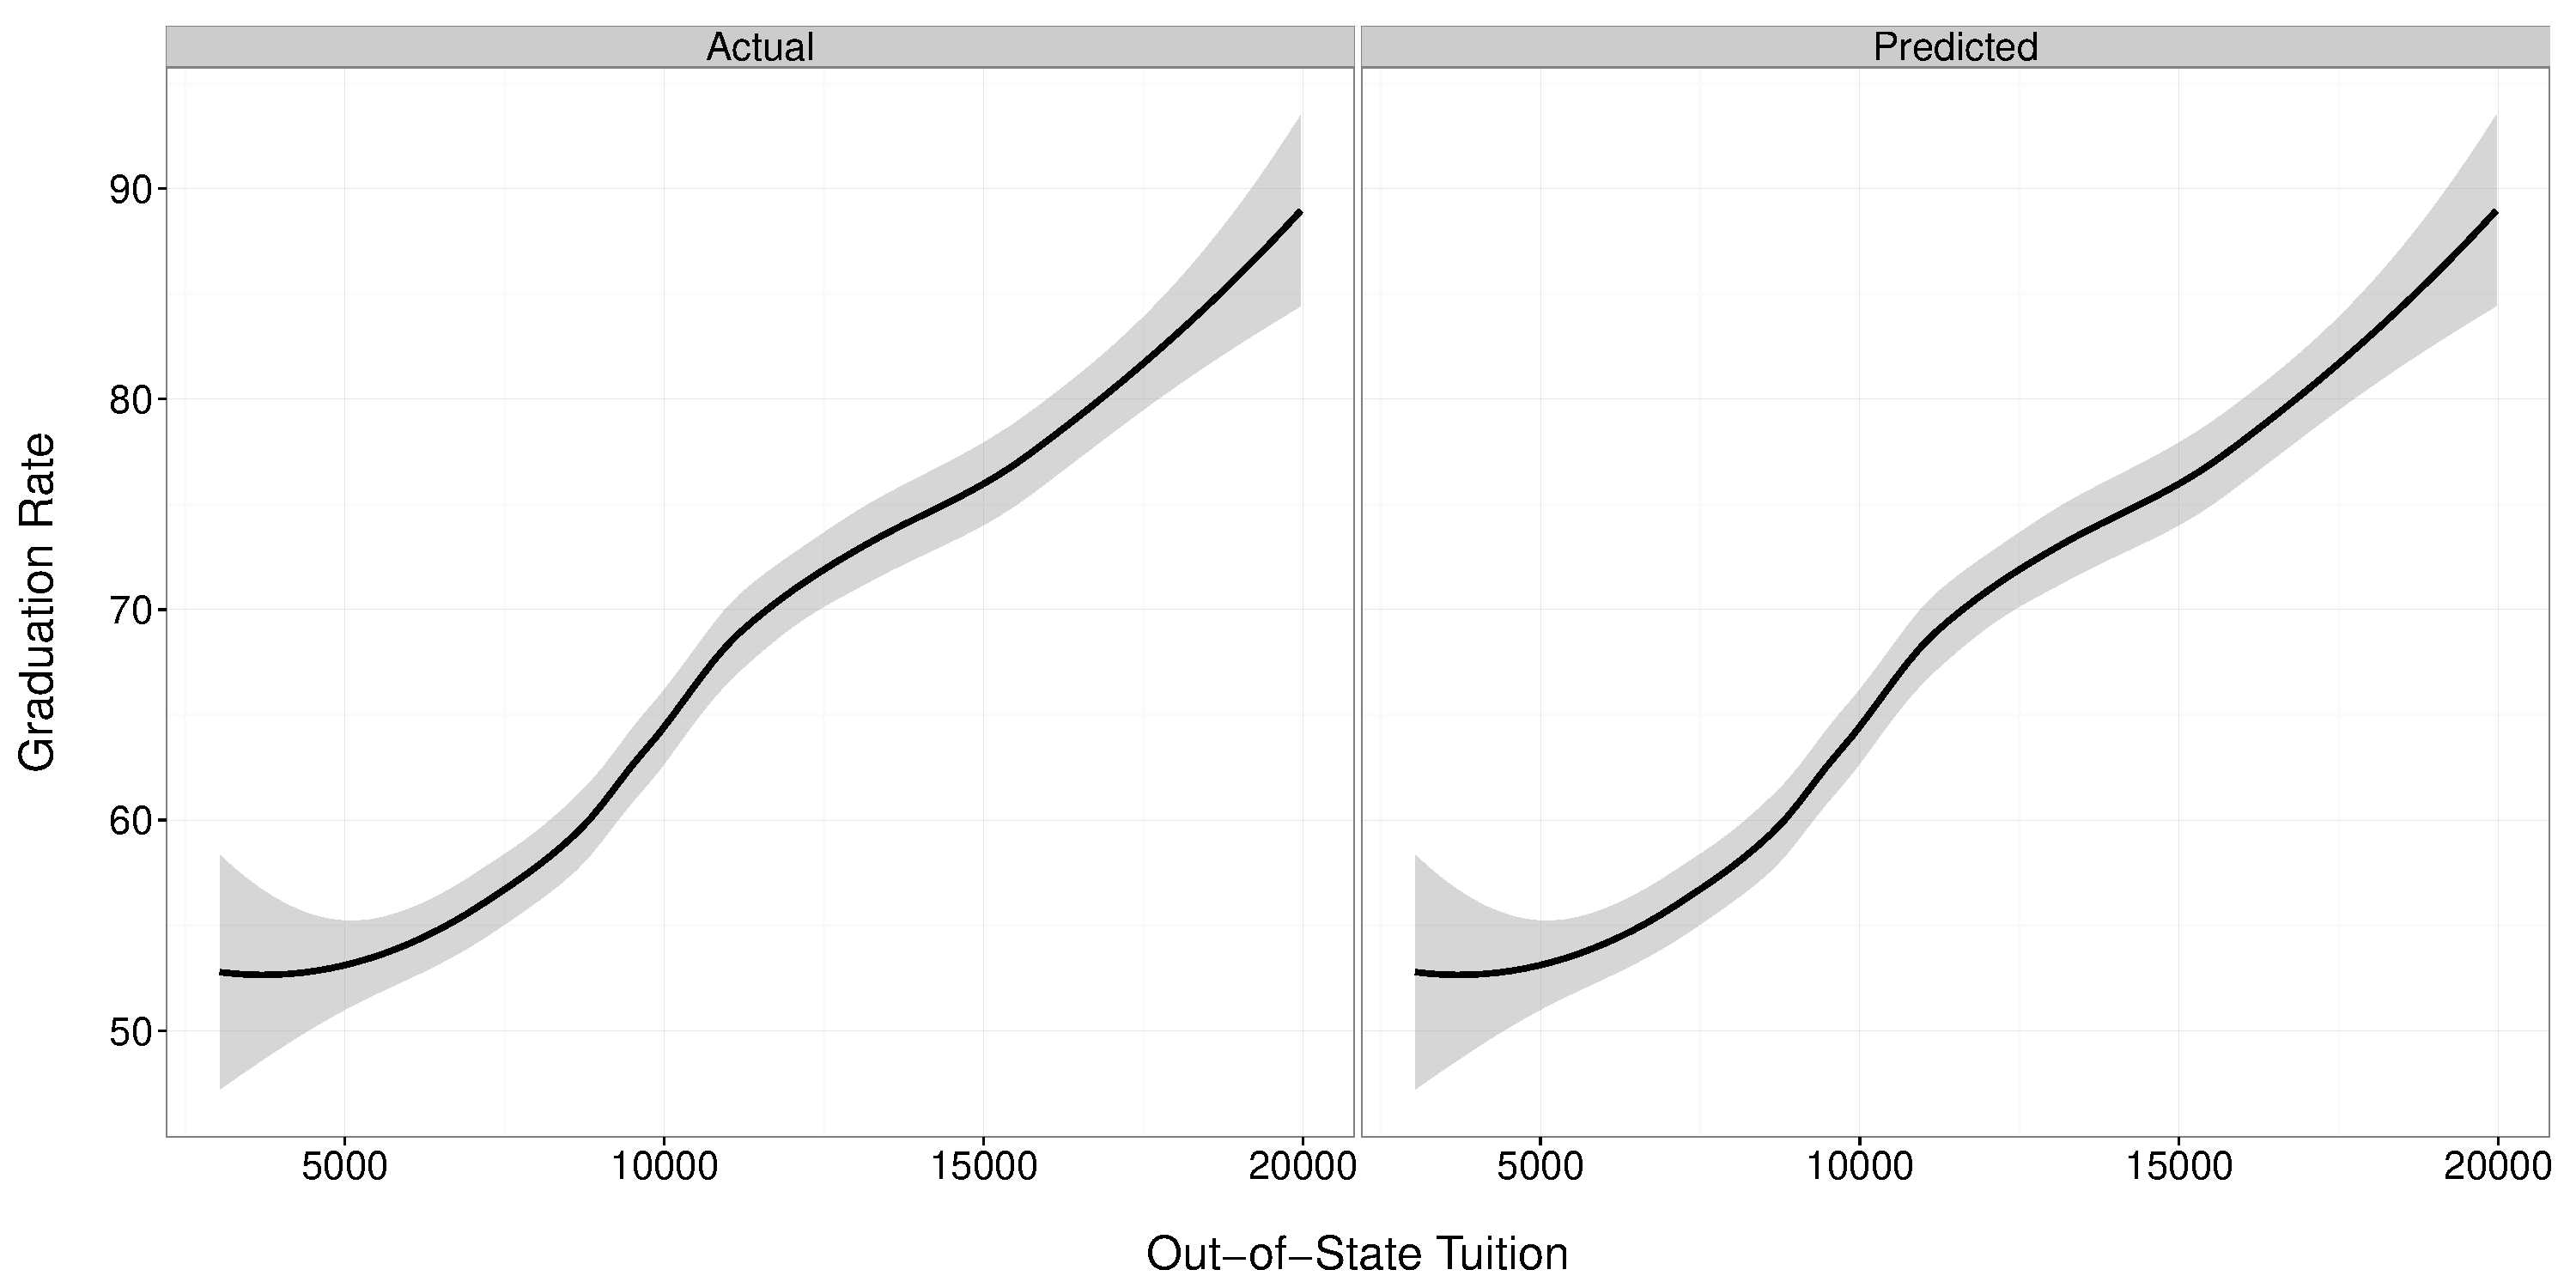
\includegraphics[width=4.5in]{Figures/Chapter02/testcheck_plot.pdf}
  \caption[Comparing the actual relation between out-of-state tuition with the relationship that was predicted with the random forest model.]{\textit{Plot comparing the actual relation between out-of-state tuition (left) with the relation that was predicted from the random forest model (right). In this case, the random forest is doing an excellent job at approximating the true functional form.}}
  \label{fig:testcheck}
\end{figure}



%----------------------------------------------------------------------------------------

\subsection{Conditional inference forests}

	In this overview so far, only a random forest with CART as the underlying partitioning algorithm has been used. In fact, random forests are easily generalizable to any recursive partitioning framework. In the case of conditional inference, for example, creating an ensemble of conditional inference trees is known as a conditional inference forest \cite<CFOREST;>{hothorn2006survival}, and can be readily adapted with one slight alteration to the original forest algorithm. Because the framework of conditional inference assumes independence, taking a bootstrap sample results in a new data set with repeated observations, thus breaking this assumption. In order to maintain an unbiased splitting procedure, this issue can solved by sampling 63.2\% of the data without replacement instead of bootstrapping (i.e., subsampling). This improvement has shown to yield an unbiased splitting procedure with predictive performance on par with CART forests \cite{strobl2007bias}. While the graphical results of the conditional inference forest will not be given for brevity, see \autoref{tab:performance} to compare the predictive performance of CART, CTREE, CART forests, and CFOREST applied to the college graduation rate data in 100 runs. Given the results of CART in \autoref{fig:tradeoff}, the tuning parameter was selected via the minimum cross-validated error rather than the 1-SE rule. Note that the performance for both trees and forests are similar between the two methods of CART and conditional inference. While this is generally true, the underlying decision tree structure will be somewhat different given the biased nature of the CART algorithm \cite{hothorn2006unbiased, strobl2007bias}. In this specific example, the top 5 predictors and their relative order (with the exception of one variable) between both random forest methods were identical.


\begin{table}
\caption[Estimated prediction performance for the four methods]{\textit{Estimated prediction performance for the four methods.}}  
\label{tab:performance}
\begin{tabular}{rcc}
\hline
Method      & Mean Performance (MSE) & SD Performance \\ \hline
CART        & 208.41                 & 19.22          \\
CTREE       & 205.28                 & 17.44          \\
CART forest & 168.61                 & 14.55          \\
CFOREST     & 169.27                 & 14.63          \\ \hline
\end{tabular}
\end{table}


%----------------------------------------------------------------------------------------

\subsection{Pros and cons of Random Forests}


	As was just shown, the major benefit to creating an ensemble of decision trees with a random forest algorithm is being able to efficiently search a large parameter space and create a predictive model that is vastly superior to single decision trees. Another added benefit is that forests are created on unpruned trees, removing the subjectivity inherently found in pruning decisions. However, this benefit of improved performance does come at the cost of reduced interpretability. While both variable importance and partial dependence plots offer ways to view the underlying structure of decision trees, these methods still mask the potential higher-order interactions underlying a given forest that are impossible to visualize. Additionally, forest methods are more computationally expensive to perform when compared to a single decision tree. This is especially true of CFOREST, which requires a more expensive permutation test framework. For example, a recent application of random forests on 876 observations with 44 variables reported 4.82 seconds for CFOREST, while CART forests only took 0.24 seconds \cite{strobl2007bias}. While this effect can be somewhat mitigated on larger data sets by the fact that forests are trivially parallelizable, this characteristic of longer computation time can be perceived as a nuisance, especially with extremely large data sets. 


%----------------------------------------------------------------------------------------

\section{Handling missing data}


	Missing data are an all-too-common occurrence in many areas of the social sciences, especially in education. Fortunately, recursive partitioning has an elegant way to handle missing data, called surrogate splits. Every time a split is made in the procedure, the algorithm automatically searches for additional variables that mimic the behavior of this main split, thus acting as a surrogate to the original variable in the case of a missing observation. These splits are derived in the exact same way as the original partitioning algorithm \cite{hothorn2006unbiased, therneau2014introduction}. More specifically, the algorithm searches for splits in other variables that best predicts membership into the two new classes created by the split in the original variable. A list of ranked variables is then created for each split in the final decision tree in case data are missing on multiple variables. While this approach seems simple, surrogate splits have been shown to yield performance similar to multiple imputation when applied to both CART and CTREE under missingness conditions that are completely at random \cite{hapfelmeier2012recursive}.


	Unfortunately, while the application of the methodology of surrogate splits can extend directly to ensembles of trees for the purpose to calculating predictions, there is no clear way to estimate permuted variable importance in the traditional way. This is one reason as to why surrogate splits are not employed in many CART forest algorithms \cite<e.g.,>{liaw2002classification, pedregosa2011scikit}. Instead, random forests often use imputation methods. For example, the original random forest algorithm employs an imputation method that iteratively builds random forests in order to impute missing values \cite{breiman2001random}. To do this, missing values are first replaced by the median of that variable (in the continuous case) or the category with the highest prevalence (in the categorical case) of that particular variable. Then, a random forest is run, and the missing values are replaced based on their proximity to other observations. That is, when a missing value is present, observations are identified that typically appear in the same nodes as this missing value in many of the trees created during the random forests process. These observations are then used to impute the missing values. This procedure is repeated a few times to iteratively improve on the final imputations. This method has also been shown to yield good performance even with higher rates of missingness (i.e., > 50\%), though it has been noted that the OOB error estimate tends to be slightly optimistic with imputed values \cite{breiman2003manual}. Note that this method only works when covariates are missing, however. Observations with the outcome missing must be either removed or imputed with a separate process.


	CFOREST utilizes surrogate splits and employs a new variable importance measure to allow the estimation of variable importance in the presence of missing data \cite{hapfelmeier2014new}. This new measure is essentially identical to permuted variable importance, with one exception. Rather than randomly permuting a variable to break its link with the outcome, observations are randomly sent to either the left of the right child node of any split that includes the variable of interest. This still breaks a variable's link with the outcome, but now the calculation of variable importance can be accomplished as before. This new technique shows a number of desirable properties over MCAR, MAR, and NMAR data, such as not yielding artificially inflated variable importance values for variables with high rates of missingness, which can occur with complete case analysis \cite{hapfelmeier2014new}. 


%----------------------------------------------------------------------------------------

\section{Other predictive methods}

	Note that recursive partitioning was specifically chosen as the focus of this dissertation given that it is nonparametric in nature, relatively easy and intuitive to understand, and their ensemble method counterparts (i.e., forests) consistently shows good performance in predictive tasks when compared to other popular methods \cite{caruana2006empirical}. However, these methods are certainly not a ``silver bullet'' for exploratory data analysis or predictive modeling in general. For example, while recursive partitioning will estimate potential non-linear relationships, linearity is often a valid assumption to make in many statistical applications. Regularized regression methods that include a penalty term in its estimation procedure, such as the L2 norm (i.e., the sum of the squared, standardized parameter estimates) in the case of ridge regression or the L1 norm (i.e., the sum of the absolute value of the standardized parameter estimates) in the case of the LASSO, can be attractive options to reduce overfitting in linear models at the small cost of increased bias \cite{hastie2009elements}. Still, extending these methods into a mixed-effects framework is a much more complicated task given the underlying assumptions of regression models, though some solutions do exist \cite<e.g.,>{eliot2011ridge, schelldorfer2011estimation}.







 % Chapter 2
% Chapter 3

\chapter{Recursive Partitioning and Multilevel Data} % Chapter title

\label{ch:previous} % For referencing the chapter elsewhere, use \autoref{ch:previous} 

	There is a small, but growing body of research that examines the application of decision trees to complex data structures. \citeA{segal1992tree} provides an initial foray into this topic by attempting to extend the logic of decision trees and covariate splits to longitudinal data. In this method, split functions for trajectories can be directed toward either the mean vector (e.g., an intercept and a slope term) or the covariance matrix. One large difficulty in this procedure is the handling of time-varying covariates. Because changes in the covariance structure is considered in the splitting function, potential splits can only be done at the participant level and not the observation level. Thus, time-varying covariates can only be included if they are aggregated to the participant-level of analysis as a low-order polynomial term. That is, using an intercept and slope to approximate the trajectory of the time-varying covariate, and then using these new variables as potential variables to split on \cite{segal1992tree}. This is an important methodological consideration that will manifest itself throughout this discussion of previous research.


	This method can also be utilized to identify representative curves for the purpose of exploratory data analysis \cite{segal1994representative}. While just sampling curves can be problematic in a sense that potential non-representative trajectories are selected (i.e., outliers), this method can detect homogeneous sub-populations of trajectories in regard to both the outcome and a set of covariates. A similar approach can be made from an unsupervised perspective, where representative groups are selected based on trajectories only and not the covariates themselves \cite{martin2014growth, tucker1966}.


	Other methods focused on applying recursive partitioning to longitudinal data employed improved algorithms that do not exhibit the selection bias commonly found in some recursive partitioning algorithms, such as CART. For example, \citeA{eo2013tree} proposed a recursive partitioning algorithm based on GUIDE \cite{loh2002regression}, which utilizes residual analysis to avoid selection bias in its splitting procedure and a cost-complexity stopping rule instead of cross-validation to save on computation time. Similar to \citeA{segal1992tree}, this method can only identify trends, not predict future responses. As such, it is limited in only being able to split on variables at the cluster level, not the observation level. A similar method proposed by \citeA{loh2013regression} also utilized GUIDE for this purpose.


	Note that these aforementioned methods focused on exploratory data analyses in a multilevel framework that is longitudinal in nature (i.e., repeated observations nested within participants). Emphasis is also being placed on predictive accuracy in a multilevel framework that is typically cross-sectional in nature. For example, \citeA{karpievitch2009introspective} examined the classification performance of random forests in mass spectrometry-based studies, which often produces cluster-correlated data. Via simulation, they found that traditional random forest algorithms yielded good classification performance despite the presence of cluster-correlated data, except that the OOB error rate typically underestimated the actual error rate calculated on a separate test data set. By extending the original random forest algorithm to instead re-sample at the cluster level rather than the observation level led to near identical median classification rates and variable selection accuracy when compared to the original random forest algorithm, but without the bias found in the OOB error rate. The conceptual background for why this occurs will be addressed in \autoref{ch:problem}.  


	Additional examples that also focus on the performance of resampling methods for random forests in cluster-correlated data are typically found in medical research. In one example, \citeA{adler2011ensemble} compared different resampling methods for random forests in the presence of paired organ data, and found that the decrease in performance at high correlations between organs can be reduced if a paired bootstrap is performed. It has also been reported that sampling one observation rather than resampling all observations within an individual can lead to better performance when classifying future observations of patients in a longitudinal framework \cite{adler2011classification}.


	More recently, researchers have also begun to focus on estimating and using a random effects structure in tandem with decision trees to improve predictions. For example, both \citeA{sela2012re} and \citeA{hajjem2011mixed} independently proposed the same method to incorporate a given random effects structure in a recursive partitioning algorithm, called RE-EM trees and mixed-effects regression trees, respectively. Both approaches operate on the same algorithm, namely one that uses a variant of the EM algorithm to estimate a set of random effects (most commonly just random intercepts) to encompass an entire tree. While any underlying decision tree algorithm can be used, both authors adopted an approach using CART. Because these random effects can be used to alter predictions for each individual observation in the sample after filtering through the tree structure, both methods show increased in-sample predictive accuracy compared to both a traditional multilevel model with main effects or a decision tree without this random effect structure. However, because random effects have a mean of zero, the predictive performance for observations nested within unobserved clusters between a decision tree with and without a random effects structure was similar \cite{hajjem2011mixed, sela2012re}.


	\citeA{hajjem2014mixed} have also extended these trees to create an ensemble method referred to as mixed-effects random forests. This method first removes the estimated random effects in the model before performing bootstrapping to avoid employing a cluster bootstrap. It also finds substantial improvements over single decision trees both with or without random effects in terms of prediction accuracy. Given the bias inherent in the splitting procedure of the CART algorithm, these methods have also been built around conditional inference trees, resulting in unbiased variable selection with the added benefit of having a random effects structure to improve predictive accuracy. Despite the unbiased variable selection, the conditional inference tree with random effects still yields similar predictive accuracy when compared to a CART tree with random effects \cite{fu2014unbiased}; a similar scenario to how these methods perform without a random effects structure \cite{strobl2007bias}.

	Additional research has investigated decision trees in multilevel contexts from a model-based perspective. That is, rather than focus on prediction with a basic tree approach where each node just represents a different mean value (in the case of a regression tree) or class (in the case of a classification tree), an alternative is to have a statistical model in each node \cite{zeileis2008model}. For example, a linear regression tree searches the covariate space for potential splits that maximizes the difference in model parameters in an already specified model. Thus, it becomes possible to unite confirmatory and exploratory research and examine potential model misspecification in more detail \cite{kopf2010potential}. Recently, model-based decision trees have been extended to a structural equation modeling (SEM) framework, called SEM trees \cite{brandmaier2013structural}. In this method, decision trees are combined with the flexibility of SEM, where SEMs are split based on a set of covariates, effectively creating a series of more homogenous multi-group models. This model-based recursive partitioning method also avoids selection bias with a two stage procedure found in \citeA{loh1997split}, which first selects the best cut point for each variable and then selects the best split among these candidates. Like many trees methods, creating an ensemble (i.e., a SEM forest) helps to reduce bias and increase the stability of estimated relationships among variables \cite{prindle2014}. Because this framework also estimates variance components, it is limited to only splitting on cluster level variables in the presence of clustered data. 

 % Chapter 3
% Chapter 4

\chapter{The Problem} % Chapter title

\label{ch:problem} % For referencing the chapter elsewhere


	As shown in the previous section, extending the recursive partitioning framework to a variety of multilevel contexts has received much research attention, especially in the last few years. However, many questions remain unanswered with regard to the application of these methods in the social sciences. For one, this previous research is typically focused solely on predictive accuracy, rather than the data-driven identification of potential variables of interest in an exploratory context. To this extent, many of these previous examples attempt to extend recursive partitioning methods to very situational circumstances, inevitably making them less flexible. Moreover, many of these simulation studies mimic the data generating process found in scientific areas where these methods are common (e.g., genomics) that are often quite different than what is found in the social sciences more generally, and education specifically. In fact, no studies previously mentioned have actually examined the original non-parametric methods outlined in \autoref{ch:methods} in multilevel contexts commonly found in education research. As such, the performance of these methods with regard to surrogate splits, selection bias, and variable importance accuracy as applied to education data is not well understood. Below, I outline three questions that manifest themselves conceptually when considering the application of recursive partitioning methods to multilevel contexts commonly found in education research. 


%----------------------------------------------------------------------------------------

\section{CART level-2 variable selection}


	Given the non-parametric nature of the CART algorithm, it would seem as though CART can be applied to multilevel contexts without much additional consideration. While this is mainly true, recall that the algorithm is inherently biased toward selecting variables with many potential split points. This effect could be compounded when considering whether the variable under consideration appears at the first level or the second level of analysis. With $N$ observations nested within $K$ clusters, the number of potential split points for a numeric variable (with no repeated values) at the first level will be $N - 1$, while the number of splits for the same variable at the second level will be $K - 1$. It is clear that if both of these variables have no relationship with the outcome, the variable measured at the lowest level will be selected more often purely due to chance. 


	The categorical case, however, will not be as affected by this methodological issue assuming the clusters have the same number of observations. For a simple example, assume we are interested in measuring the entropy of a node that has a sample size of 16 (four observations nested within four clusters), along with a variable that is dichotomous. Suppose there exists a 50 percent chance of belonging into one outcome group versus the other. Because the observations are balanced within each cluster, the entropy of both situations is identical, regardless of whether the group was assigned at the cluster level or the observation level. 


%----------------------------------------------------------------------------------------

\section{The breakdown of conditional inference}


	As mentioned previously, conditional inference trees assume data that are independent. Thus, the splitting procedure will be more likely to select a split in the presence of cluster-correlated data (i.e., an increased chance of a false positive for splitting), resulting in a tree that is more likely to overfit due to being too complex. Preliminary simulations indicate that while varying the level of the variation in the outcome due to the cluster-level (i.e., the intra-class correlation coefficient, or ICC) can result in some bias, the conditional inference procedure is most affected by the presence of non-independence due to the inclusion of level-2 variables in the splitting procedure. This follows conceptually from traditional regression techniques, where standard error inflation most often occurs due to the presence of level-2 variables incorporated at the first level of analysis \cite{luke2004multilevel}. 


	Despite this methodological issue, conditional inference trees may still be useful in certain situations. For example, the rate of alpha inflation on data sets with only level-1 variables may result in trees that are still unbiased with respect to their splitting criteria, but just overfit the data due to non-independence. Simply altering the complexity parameter with cross-validation could be a potential solution to this issue. Additionally, trees are typically grown to maximum depth when creating a random forest. Conditional inference forests might still yield good predictive performance in the presence of non-independence, because conditional inference trees will have much more complexity in this case, which is removed in the aggregation procedure found in random forests. Regardless, many researchers might not realize the assumptions inherent to conditional inference trees, and inappropriately apply this method in multilevel contexts. Thus, it is important to identify situations where conditional inference is completely unreliable and where it might still be useful.


%----------------------------------------------------------------------------------------

\section{Underestimating OOB error}


	In the random forest methodology, recall that approximately 37\% of all observations in a sample will not be chosen in each bootstrap, referred to as the OOB sample. In a cluster-correlated sample, however, observations within a given cluster are more related to other observations within that cluster compared with observations in other clusters. Thus, exposing a tree to a given observation within a cluster actually informs the tree about other observations within that same cluster. This results in trees that are correlated with one another, yielding an OOB error estimate that is overly optimistic \cite{karpievitch2009introspective}. This is most problematic when the intra-class correlation (ICC) is high, something not commonly found in cross-sectional multilevel models in education. 
Both previous research \cite<i.e.,>{karpievitch2009introspective} and preliminary simulations suggest that this methodological artifact should not be too problematic with smaller ICC values. In other areas where higher ICCs are common (e.g., mass spectrometry), other non-parametric bootstrap methods might provide a more reliable OOB error estimate. An alternative solution for a more accurate estimate of the test error without altering the re-sampling process underlying the algorithm would be to use cross-validation on the clusters rather than the observations, which has been shown to provide approximately unbiased estimates of test error in the presence of dependent data \cite{rice1991estimating, segal1992tree}.


	However, note that the OOB samples are not only used as an estimate of test error, but also used to create the permuted variable importance measures. Thus, an overly optimistic OOB error estimate could lead to additional bias being introduced to variable importance measures. Again, because this issue is not substantial when ICC values are low, I do not expect much bias in the variable importance measures to occur. Regardless, this issue remains an open question, and will be investigated more thoroughly in this dissertation. 

 % Chapter 4
% Chapter 5

\chapter{The Proposal} % Chapter title

\label{ch:proposal} % For referencing the chapter elsewhere, use \autoref{ch:proposal} 

With the quantitative issues outlined above, the behavior of CART, CTREE, CART forests and CFOREST need to be better understood in multilevel contexts before they can be used as exploratory data analytic tools in education research. Additionally, because the knowledge of these techniques among substantive researchers in the social sciences is limited, sharing this dissertation with these researchers to highlight the potential utility of these methods is of the utmost importance. As such, this dissertation will not only include a simulation and application phase, but also include a dissemination phase. 


%----------------------------------------------------------------------------------------

\section{Simulation phase}

The goal of the simulation phase is to evaluate the performance of recursive partitioning methods in situations commonly found in education research and identify where these techniques may or may not be reliable. Naturally, given the inherent complexities of multilevel data and the many unanswered questions outlined in the previous section, these techniques will not be perfect. However, this does not mean that they will not be useful. In total, six parameters are of interest and can potentially be manipulated in the simulation study.


The first two, number of levels in the data generation process and nature of the outcome, will be fixed to keep this simulation from becoming too unwieldy. The number of levels will be fixed to two for simplicity, while the nature of the outcome will be fixed to be continuous. Simulation research regarding recursive partitioning methods often do this as a simplifying step, finding that the results of continuous (or categorical) outcomes often generalize to the other condition \cite<e.g.,>{strobl2007bias}. The first parameter of interest to vary is sample size, which can systematically vary at two possible levels of analysis in the context of a two-level design. Common values can also be quite different depending upon the sample and research questions. For example, a limiting factor for sample size in some education research is the number of units at the first level of analysis (e.g., children in a classroom, or teachers in a school). In the same vein, however, it might be easier to collect units at the first level (e.g., students in a school). To reflect this potential variability, four categories have been chosen: 5/20, 15/20, 15/100, 100/50, where the first value corresponds to the level-1 sample size, and the second value corresponds to the level-2 sample size. Thus, the total sample size for each condition is the product of the relative sample sizes at each level. These values were chosen to range from a small-scale study with a limited sample size at both levels, to a larger scale study with a large sample size for both levels. 

The second parameter to be varied is the intraclass correlation coefficient (ICC), which reflects the proportion of variance in the outcome that is attributable to the second level of the analysis. \citeA{peugh2010practical} reports that education research typically reports ICCs ranging from 0.05 to 0.20. To reflect these common values, three categories were selected for this parameter: 0.0, 0.15, and 0.30. An ICC of 0.0 corresponds to data that are independent, an ICC of 0.15 is meant to act as an average ICC level found in educational research, while an ICC of 0.30 is meant to represent a large ICC level found in educational research.

The third parameter to be varied is the amount of missingness in the covariates. While the mechanism behind missing data can be complex \cite<e.g.>{rubin1976inference}, this study will only implement data that are missing completely at random. Because of the non-parametric nature of these algorithms and their built-in methods to handle missing data, recent research has found that simulation results for data that are missing completely at random are very similar to results with more complicated missingness mechanisms \cite{hapfelmeier2012analysis, rieger2010random}.  Missingness will be set at three possible categories for all covariate values: 0\%, 10\%, and 30\%. These values are meant to represent missingness percentages that I believe to be small, moderate, and large in the context of educational data sets.

Finally, the level at which the covariates are measured will also be manipulated. Given that preliminary simulations showed potential issues with level-2 variables, the variables will be simulated to be either level-1 only, or both level-1 and level-2. A condition with only level-2 variables is not needed, as such an analysis typically aggregates the outcome to the second level, creating a new data set that is no longer multilevel in nature. Thus, with a fully-crossed simulation design, there are 96 (4 x 3 x 4 x 2) simulation conditions. Each unique condition will be run 200 times for a total of 19,200 data sets in total. With four predictive models (CART, CTREE, CART forest, and CFOREST), 76,800 models will be run for this dissertation. See \autoref{tab:conditions} for a summary of the parameters to be manipulated in this study.

\begin{table}
\caption[The parameters to be manipulated in the simulation study.]{text\it{The parameters to be manipulated in the simulation study.}}  
\label{tab:conditions}
\begin{tabular}{rcc}
\hline
Simulation Parameter & \begin{tabular}[c]{@{}c@{}}Number of\\ Categories\end{tabular} & Category Values             \\
\hline
Number of levels & 1 & 2 \\
Nature of outcome & 1 & continuous \\
Sample size (L1/L2) & 4 & 5/20, 15/20, 15/100, 100/50 \\
Intra-class correlation & 3 & 0, 0.15, 0.30 \\
Missingness (MCAR)     & 3 & 0, 10\%, 30\% \\
Covariate level & 2 & level-1 only, both levels   \\
\hline
\end{tabular}
\end{table}

%----------------------------------------------------------------------------------------

\section{Application phase}

In order to convey the utility of these methods and implement the knowledge learned from the simulation phase, exploratory data analysis using recursive partitioning will be performed on three real data sets. These data sets all vary with regard to methodological characteristics, which will help make the proposed application of recursive partitioning more generalizable. The first data set is derived from the multilevel package in R \cite{multilevelR}. A total of 7,185 students are nested within 160 schools, where the outcome of interest is student math achievement. Possible predictor variables include number of students in the school, whether the school is public or Catholic, and the various demographic characteristics of the students. This data set is a good first application due to its simplicity, large sample size, and the fact that it has no missing data.


The second data set was derived from the Responsive Classroom Efficacy Study, which examined the impact of a social and emotional learning intervention \cite{rimm2013efficacy}. With 139 teachers nested within 24 schools (13 treatment, 11 control), Rimm-Kaufman et al. (2014) found that fidelity of implementation of this training program was shown to be an important factor relating to student achievement. In this current study, recursive partitioning methods will be used to explore possible baseline teacher or school characteristics that might be related to how these teachers implemented the training. Possible variables of interest include teacher self-efficacy in instruction and classroom management, and their attitudes toward their principal, schools programs, and teaching in general. This data set offers unique methodological challenges with a smaller sample size, moderate rates of missingness, and a continuous outcome.


The last data set is derived from the first year of a randomized field trial of a coaching intervention for teachers \cite{allen2011interaction}. A total of 960 students and 68 different teachers participated in this study, with 62\% of students belonging to middle school. The classes were split across Math (33\%), English (32\%), History (21\%), and Science (14\%). The focus of this exploratory analysis is to identify potential student-level or teacher-level variables that relate to student achievement at the end of the year. Potential variables include: student-report measures (such as motivation, engagement, peer relationships, and perspective of teacher-student relationships), teacher-report measures (such as opinions of professional development, improving student learning, their own emotional well-being, and stress), and teacher instruction quality (using an observationally based measure collected eight times throughout the year). This data set offers unique methodological challenges, with a much larger sample size, minimal missing data, longitudinal measures, and a categorical outcome (i.e., student proficiency on a standardized test).


%----------------------------------------------------------------------------------------

\section{Dissemination phase}

	After the previous two phases have been completed, this dissertation will disseminate the findings to applied educational researchers. First, an R package will be created to house useful code to assist in the analysis of decision trees on multilevel data. This package will be publicly available for download and installation on my GitHub profile, and include functions that split the data set into training and test data at the second level of analysis, perform cross-validation at the second level to give a better approximation of test error for the purpose of tuning tree and forest hyper-parameters, and perform helpful and efficient graphic visualizations of the tree and forest data structures. One such visualization example is the need for an efficient implementation of two-dimensional partial dependence plots for random forests, which is currently not available in the R computing environment. 


	In addition to this R package, a small workshop will be given to approximately five quantitatively-oriented substantive researchers here in the Curry School of Education interested in data mining. This small workshop will include an overview of recursive partitioning methods and outline a set of best practices to keep in mind when applying these methods to multilevel data. Then, after walking through the results and analysis of the first applied example on math achievement, those attending the workshop will have a chance to apply recursive partitioning methods to their own data using the R package I created, hopefully uncovering insights along the way. Feedback from this workshop will be used to alter the R package and tutorial that was created in order to make it more accessible.


%----------------------------------------------------------------------------------------

\section{Timeline}

	I will begin working on what I propose in February, with the goal completion date set at the end of the summer. My proposed seven-month timeline is as follows. The first month will be dedicated to writing the simulation scripts. Because my preliminary simulation scripts serve as a good foundation for what I need to accomplish, this will give me adequate time to test my parameter manipulations and make alterations if necessary. The second month will be spent running and interpreting the simulation results. Assuming an average computation time per model of 1 second, these simulations will take about 21 hours to complete. However, I plan on utilizing the University's Linux cluster, where I have access to multiple cores. With access to 20 cores, these simulations will be cut down to about one hour in total. Even an extremely conservative estimate of increasing the computation time to 10 seconds per model will yield a computation time of approximately 10 hours; a reasonable amount of time for these simulations to be completed overnight.


	After the interpretation of these simulation results, the next month will be spent analyzing the three application data sets using a set of best practices derived from what I learned from the simulation results. While the initial analyses will not require much time, the majority of this month will be spent working with the researchers who originally collected these data in the latter two applied examples in order to interpret and write-up the results. The following month will be dedicated to creating an R package that houses the useful code I have used for this dissertation, which will be openly available for anyone to install and use on their own computers. This month will also be spent preparing the small workshop to give to applied researchers. By the end of the month, I hope to give the workshop with the code ready to be used for illustrative purposes. The next month will be spent writing up the final results and incorporating the qualitative feedback collected during the workshop, culminating in my dissertation defense in the following month. This timeline gives approximately a month of overhead in the case of unforeseen complications. See \autoref{fig:timeline} for a graphical depiction of this timeline.

\begin{figure}[hb]
  \centering
  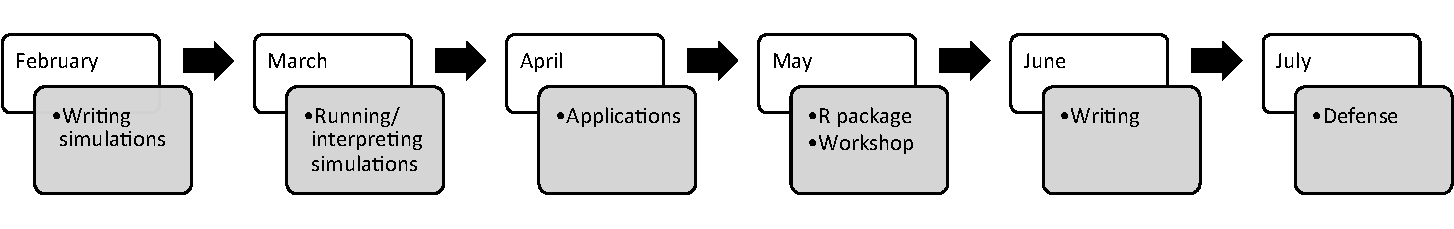
\includegraphics[width=4.5in]{Figures/Chapter05/timeline.pdf}
  \caption[My proposed dissertation timeline.]{\textit{My proposed dissertation timeline.}}
  \label{fig:timeline}
\end{figure}

%----------------------------------------------------------------------------------------

\section{Conclusion}

	To conclude, recursive partitioning methods provide an efficient way to perform exploratory data analysis in the social sciences. However, the behavior of these methods when multilevel data are present is not well understood. For my dissertation, I propose examining the performance of these methods under various simulation conditions commonly found in education research. With what I learn from the simulation results, I will apply these methods to three real data sets in order to perform exploratory data analysis in a data-driven way. Following this, I will create and share an R package and a set of best practices to help applied researchers implement these analytic tools in their own research. With this proposal, I hope to highlight the potential benefits of using recursive partitioning methods for efficient exploratory data analysis in the social sciences, especially with regard to multilevel applications in education research. 

 % Chapter 5

%----------------------------------------------------------------------------------------
%	THESIS CONTENT - APPENDICES
%----------------------------------------------------------------------------------------

%\appendix

%\part{Appendix} % New part of the thesis for the appendix

%\include{Chapters/Chapter0A} % Appendix A
%\include{Chapters/Chapter0B} % Appendix B - empty template

%----------------------------------------------------------------------------------------
%	POST-CONTENT THESIS PAGES
%----------------------------------------------------------------------------------------

% Bibliography

\label{app:bibliography} % Reference the bibliography elsewhere with \autoref{app:bibliography}

\manualmark
\markboth{\spacedlowsmallcaps{\bibname}}{\spacedlowsmallcaps{\bibname}} 
\refstepcounter{dummy}

\addtocontents{toc}{\protect\vspace{\beforebibskip}} % Place the bibliography slightly below the rest of the document content in the table of contents

\bibliographystyle{apacite}

\bibliography{Bibliography} % Bibliography

%\include{FrontBackMatter/Colophon} % Colophon

%\cleardoublepage\include{FrontBackMatter/Declaration} % Declaration

%----------------------------------------------------------------------------------------

\end{document}
